\subsection{The integral closure of a ring of fractions}

Let A be a ring, R an A-algebra and S a multiplicative subset of A. Recall (Chapter II, § 2, no. 8) that \(\mathbf{S}^{-1}\mathbf{R}\) has a canonical \(\mathbf{S}^{-1}\mathbf{A}\) -algebra structure.

PROPOSITION 16. Let A be a ring, R an A-algebra, A' the integral closure of A in R and S a multiplicative subset of A. Then the integral closure of \(\mathbf{S}^{-1}\mathbf{A}\) in \(\mathbf{S}^{-1}\mathbf{R}\) is \(\mathbf{S}^{-1}\mathbf{A}'\) .

Let \(b / s\) be an element of \(S^{-1}A'\) ( \(s \in S, b \in A'\) ). Since the diagram

\pandocbounded{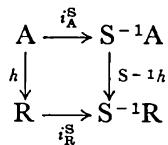
\includegraphics[keepaspectratio]{images/part002_55e4c379.jpg}}

is commutative, \(b / 1\) is integral over \(S^{-1}A\) (no. 1, Proposition 2). As \(1 / s \in S^{-1}A\) , \(b / s = (b / 1)(1 / s)\) is integral over \(S^{-1}A\) .

Conversely, let \(r / t\) ( \(r \in \mathbb{R}\) , \(t \in \mathbb{S}\) ) be an element of \(\mathbf{S}^{-1}\mathbf{R}\) which is integral over \(\mathbf{S}^{-1}\mathbf{A}\) ; then \(r / 1 = (t / 1)(r / t)\) is integral over \(\mathbf{S}^{-1}\mathbf{A}\) . Then there is a relation of the form

\[
(r / 1) ^ {n} + (a _ {1} / s) (r / 1) ^ {n - 1} + \dots + (a _ {n} / s) = 0,
\]

where \(a_{i} \in \mathbf{A}\) ( \(1 \leqslant i \leqslant n\) ) and \(s \in \mathbf{S}\) . This relation may also be written

\[
(s r ^ {n} + a _ {1} r ^ {n - 1} + \dots + a _ {n}) / s = 0
\]

and therefore there exists \(s' \in S\) such that \(s'^{n}(sr^{n} + a_{1}r^{n-1} + \cdots + a_{n}) = 0\) ; we deduce that \((s'sr)^{n} + s'a_{1}(s'sr)^{n-1} + \cdots + s'^{n}s^{n-1}a_{n} = 0\) . By definition therefore \(s'sr \in A'\) , whence \(r/1 \in S^{-1}A'\) and \(r/t \in S^{-1}A'\) .

COROLLARY 1. Let A be an integral domain, A' its integral closure and S a multiplicative subset of A such that \(0 \notin S\) . Then the integral closure of \(S^{-1}A\) is \(S^{-1}A'\) .

The field of fractions R of A is also the field of fractions of \(S^{-1}A\) since \(0 \notin S\) (Chapter II, § 1, no. 1, Remark 7); Proposition 16 is then applied to R.

COROLLARY 2. Let A be an integral domain, K its field of fractions, R an algebra over K and B the integral closure of A in R. The elements of R which are algebraic over K (no. 1, Example 1) are the elements of the form \(a^{-1}b\) where \(b \in \mathbf{B}\) and \(a \in \mathbf{A}\) , \(a \neq 0\) ; if L is the algebraic closure of K in R, there exists a basis of L over K contained in B.

The first assertion follows from Proposition 16 applied in the case \(\mathbf{S} = \mathbf{A} - \{0\}\) . If \((x_{i})_{i\in I}\) is a basis of \(\mathbf{L}\) over \(\mathbf{K}\) , then there exists for all \(i\in I\) an element \(a_{i}\neq 0\) of \(\mathbf{A}\) such that \(a_{i}x_{i}\in \mathbf{B}\) ; then \((a_{i}x_{i})_{i\in I}\) is also a basis of \(\mathbf{L}\) over \(\mathbf{K}\) .

COROLLARY 3. Let A be an integral domain and \(\Omega\) the set of maximal ideals of A. For A to be integrally closed, it is necessary and sufficient that, for all \(\mathfrak{m} \in \Omega\) , \(\mathbf{A}_{\mathfrak{m}}\) be integrally closed.

It follows from Corollary 1 that the condition is necessary. The condition is sufficient, for \(\mathbf{A} = \bigcap_{m \in \Omega} \mathbf{A}_m\) (Chapter II, §3, no. 3, formula (2)) and it is sufficient to apply the Corollary to Proposition 8 of no. 2.

COROLLARY 4. Let A be an integral domain, K its field of fractions and S a multiplicative subset of A such that \(0 \notin S\) .

\begin{enumerate}
\def\labelenumi{(\roman{enumi})}
\item
  Let B be a subring of K which is integral over A and let f be the annihilator of the A-module B/A. Then \(S^{-1}f\) is contained in the annihilator of the \((S^{-1}A)\) -module \(S^{-1}B/S^{-1}A\) and is equal to this annihilator if B is a finitely generated A-module.
\item
  Let A' be the integral closure of A. For \(S^{-1}A\) to be integrally closed, it is sufficient that the annihilator f of the A-module A'/A meet S. This condition is also necessary if A' is a finitely generated A-module.
\setcounter{enumi}{0}
\item
  As \(\mathfrak{f}\mathbf{B} \subset \mathbf{A}\) , \((\mathrm{S}^{-1}\mathfrak{f})(\mathrm{S}^{-1}\mathbf{B}) \subset \mathrm{S}^{-1}\mathbf{A}\) and hence \(\mathrm{S}^{-1}\mathfrak{f}\) is contained in Ann \((\mathrm{S}^{-1}\mathrm{B} / \mathrm{S}^{-1}\mathrm{A})\) . If \(\mathbf{B}\) is a finitely generated A-module, the equation \(\mathrm{S}^{-1}\mathfrak{f} = \operatorname{Ann}(\mathrm{S}^{-1}\mathrm{B} / \mathrm{S}^{-1}\mathrm{A})\) is a special case of formula (9) of Chapter II, § 2, no. 4, \(\mathrm{S}^{-1}\mathrm{B} / \mathrm{S}^{-1}\mathrm{A}\) being canonically identified with \(\mathrm{S}^{-1}(\mathrm{B} / \mathrm{A})\) .
\item
  By Corollary 1 \(\mathbf{S}^{-1}\mathbf{A}'\) is the integral closure of \(\mathbf{S}^{-1}\mathbf{A}\) . As the relations \(\mathfrak{f} \cap \mathbf{S} \neq \varnothing\) and \(\mathbf{S}^{-1}\mathfrak{f} = \mathbf{S}^{-1}\mathbf{A}\) are equivalent (Chapter II, § 2, no. 5, Remark) (ii) is an immediate consequence of (i).
\end{enumerate}

If B is a subring of K which is integral over A, the annihilator f of B/A (equal by definition to the transporter A: B (Chapter I, § 2, no. 10)) is sometimes called the conductor of B in A.

COROLLARY 5. Let A be an integral domain, A' its integral closure and f the annihilator of the A-module A'/A. Suppose that A' is a finitely generated A-module. The prime ideals p of A such that A \(_{p}\) is not integrally closed are those which contain f.

This follows immediately from Corollary 4 (ii) applied to S = A - p.

Note that under the hypotheses of Corollary 5 f ≠ 0 since A' is a finitely generated A-module and every element of K/A (K the field of fractions of A) has an annihilator ≠ 0.

* In algebraic geometry, Corollary 5 and the above remark show that the points where an affine variety V is not normal form a closed set distinct from V. *

\subsection{Norms and traces of integers}

PROPOSITION 17. Let A be a ring, B a (commutative) A-algebra and X a square matrix of order n over B; the following properties are equivalent:

\begin{enumerate}
\def\labelenumi{(\alph{enumi})}
\item
  \(X\) is integral over A.
\item
  There exists a finitely generated sub-A-module \(\mathbf{M}\) of \(\mathbf{B}^n\) such that \(X.x\in \mathbf{M}\) for all \(x\in \mathbf{M}\) and \(\mathbf{M}\) is a system of generators of the B-module \(\mathbf{B}^n\) .
\item
  The coefficients of the characteristic polynomial of \(X\) are integral over \(\mathbf{A}\) .
\end{enumerate}

  If \(\chi(T) = \det(T.1 - X)\) is the characteristic polynomial of \(X\) , the Cayley-Hamilton Theorem shows that \(\chi(X) = 0\) (Algebra, Chapter VII, § 5, no. 4, Remark 1) and, as \(\chi\) is a monic polynomial, (c) implies (a) by no. 1, Proposition 6.

  Suppose in the second place that (a) holds. If \((e_i)_{1 \leqslant i \leqslant n}\) is the canonical basis of \(B^n\) , the sub-A-module M of B generated by the \(X^k \cdot e_i\) ( \(1 \leqslant i \leqslant n, k \geqslant 0\) ) is a finitely generated A-module, since the A-algebra A[X] is a finitely generated A-module (no. 1, Theorem 1); as M contains the \(e_i\) , it is seen that (a) implies (b); the converse is a consequence of no. 1, Theorem 1, condition \((E_{\mathrm{III}})\) .

  Finally let us prove that (a) implies (c); as X is integral over A and a fortiori over the polynomial ring A[T], T.1 - X is also integral over A[T] and by no. 3, Proposition 12 the problem is seen to reduce (by replacing X by T.1 - X and A by A[T]) to proving that, if X is integral over A, \(d = \det(X)\) is an element of B which is integral over A. Now, we have seen above that the endomorphism u of \(B^{n}\) defined by X leaves stable a finitely generated sub-A-module M containing the \(e_{i}\) ; the n-vectors \(x_{1} \wedge x_{2} \wedge \cdots \wedge x_{n}\) , where \(x_{i} \in M\)

for \(1 \leqslant i \leqslant n\) , therefore generate in \(\bigwedge (\mathbf{B}^n)\) a finitely generated sub-A-module containing \(e_1 \wedge e_2 \wedge \cdots \wedge e_n\) and which is stable under \(\bigwedge^n u\) , in other words under the homothety of ratio \(d\) ; as the annihilator of

\[
e _ {1} \wedge e _ {2} \wedge \dots \wedge e _ {n}
\]

in B reduces to 0, condition \((\mathbf{E}_{\mathrm{III}})\) of no. 1, Theorem 1 proves that \(d\) is integral over A.

COROLLARY 1. Let A be an integral domain, K its field of fractions and K' a finite-dimensional K-algebra (not necessarily commutative). If \(x \in \mathbf{K}'\) is integral over A, the coefficients of the characteristic polynomial \(\mathrm{Pc}_{\mathbf{K}' / \mathbf{K}}(x; \mathbf{X})\) (Algebra, Chapter VIII, § 12, no. 2) are integral over A.

If \(z \mapsto M(z)\) is the regular representation of the algebra \(\mathbf{K}'\) (considered as a matrix representation; cf.~Algebra, Chapter VIII, § 13) \(\mathrm{Pc}_{\mathbf{K}' / \mathbf{K}}(x; \mathbf{X})\) is by definition the characteristic polynomial of the matrix \(M(x)\) ; if \(x\) integral over \(\mathbf{A}\) , the matrix \(M(x)\) is integral over \(\mathbf{A}\) (no. 1, Proposition 2) and it is sufficient to apply Proposition 17.

COROLLARY 2. With the same hypotheses and notation as in Corollary 1, \(\mathrm{Tr}_{\mathbf{K}^{\prime}/\mathbf{K}}(x)\) and \(\mathbf{N}_{\mathbf{K}^{\prime}/\mathbf{K}}(x)\) are integral over A.

\(\mathrm{Tr}_{\mathbf{K}^{\prime}/\mathbf{K}}(x)\) and \(\mathrm{N}_{\mathbf{K}^{\prime}/\mathbf{K}}(x)\) are, to within a sign, coefficients of \(\mathrm{Pc}_{\mathbf{K}^{\prime}/\mathbf{K}}(x;\mathbf{X})\) (Algebra, Chapter VIII, § 12, no. 1, equations (4)) and hence are integral.

Remark (1) If \(\mathbf{K}'\) is a simple central algebra over \(\mathbf{K}\) and \(x \in \mathbf{K}'\) is integral over \(\mathbf{A}\) , the coefficients of the reduced characteristic polynomial of \(x\) (Algebra, Chapter VIII, § 12, no. 3) are integral over \(\mathbf{A}\) . For there is a power of this polynomial equal to \(\mathrm{Pc}_{\mathbf{K}' / \mathbf{K}}(x; \mathbf{X})\) (loc. cit., Proposition 8) and it is sufficient to apply Proposition 17 and no. 3, Proposition 11.

PROPOSITION 18. Let A be an integrally closed domain, K its field of fractions, K' a finite-dimensional separable K-algebra (Algebra, Chapter VIII, §7, no. 5) and A' the integral closure of A in K'. Then A' is contained in a finitely generated A-module.

The proposition will follow from the following more precise lemma:

LEMMA 3. Under the hypotheses of Proposition 18, let \((w_{1},\ldots ,w_{n})\) be a basis of \(\mathbf{K}'\) over \(\mathbf{K}\) contained in \(\mathbf{A}'\) (no. 5, Corollary 2 to Proposition 16); then there is a unique basis \((w_{1}^{*},\dots ,w_{n}^{*})\) of \(\mathbf{K}'\) over \(\mathbf{K}\) for which \(\mathrm{Tr}_{\mathbf{K}' / \mathbf{K}}(w_i w_j^*) = \delta_{ij}\) (Kronecker index); if \(d = \mathrm{D}_{\mathbf{K}' / \mathbf{K}}(w_1,\dots ,w_n)\) is the discriminant of the basis \((w_{1},\dots ,w_{n})\) (Algebra, Chapter IX, § 2), then \(d\neq 0\) and

\[
\sum_ {i = 1} ^ {n} \mathrm{A} w _ {i} \subset \mathrm{A} ^ {\prime} \subset \sum_ {i = 1} ^ {n} \mathrm{A} w _ {i} ^ {*} \subset d ^ {- 1} \left(\sum_ {i = 1} ^ {n} \mathrm{A} w _ {i}\right).\tag{2}
\]

In particular, if \(d\) is an invertible element of \(\mathbf{A}\) , \(\mathbf{A}'\) is a free \(\mathbf{A}\) -module with basis \((w_1, \ldots, w_n)\) .

As \(\mathbf{K}'\) is a separable K-algebra, \(d \neq 0\) (Algebra, Chapter IX, §2, Proposition 5) and the K-bilinear form

\[
(x, y) \mapsto \operatorname{Tr} _ {\mathbf {K} ^ {\prime} / \mathbf {K}} (x y)
\]

over \(\mathbf{K}'\) is therefore non-degenerate (loc. cit., Proposition 4); this shows the existence and uniqueness of the basis \((w_{i}^{*})_{1\leqslant i\leqslant n}\) (Algebra, Chapter IX, §1, no. 6, Corollary to Proposition 6). This being so, the first inclusion of (2) is

obvious. Let \(x\) be an element of \(\mathbf{A}'\) ; let us write \(x = \sum_{i=1} \xi_i w_i^*\) where \(\xi_i \in \mathbf{K}\) ; for all \(i\) , \(\xi_i = \mathrm{Tr}_{\mathbf{K}' / \mathbf{K}}(xw_i)\) , hence \(\xi_i\) is integral over \(\mathbf{A}\) (Corollary 2 to Proposition 17) and, as \(\mathbf{A}\) is integrally closed, \(\xi_i \in \mathbf{A}\) for \(1 \leqslant i \leqslant n\) ; this shows the second

inclusion (2). Finally, let us write \(w_{j}^{*} = \sum_{l=1}^{n} \alpha_{jl} w_{l}\) where \(\alpha_{jl} \in \mathbf{K}\) ; then \(\sum_{i=1}^{n} \alpha_{ji} \mathrm{Tr}_{\mathbf{K}'/\mathbf{K}}(w_i w_k) = \delta_{jk}\) for all \(j\) and \(k\) ; Cramer's formulae show that the \(\alpha_{ji}\) belong to \(d^{-1}\mathbf{A}\) , whence the third inclusion (2). The last assertion follows immediately from (2), which in this case gives \(\mathbf{A}' = \sum_{i=1}^{n} \mathbf{A}w_i\) .

In the two corollaries which follow the hypotheses and notations are those of Proposition 18.

COROLLARY 1. If A is a Noetherian ring, the A-module A' is finitely generated and in particular the ring A' is Noetherian.

A' is a submodule of a finitely generated A-module.

COROLLARY 2. If A is a principal ideal domain, A' is a free A-module of rank n.~Every submodule of a free A-module is then free (Algebra, Chapter VII, § 3, Theorem 1).

COROLLARY 3. Let E be an extension of degree n of the field Q of rational numbers. The additive group of the integral closure in E of the ring Z of rational integers is a free commutative group of rank n.

Z is integrally closed (no. 3, Proposition 10) and E is separable since Q is of characteristic 0. Corollary 2 can therefore be applied to the case where A = Z, K = Q and K' = E.

Remark (2). The conclusions of Corollary 1 are not necessarily true if \(\mathbf{K}'\) is not assumed to be separable over \(\mathbf{K}\) , even if \(\mathbf{K}'\) is an extension field of \(\mathbf{K}\) (Exercise 20). On the other hand, if \(\mathbf{A}\) is a finitely generated integral \(\mathbf{K}_0\) -algebra, where \(\mathbf{K}_0\) is a field, the integral closure of \(\mathbf{A}\) in any extension of finite degree of the field of fractions of \(\mathbf{A}\) is a finitely generated A-module and a Noetherian ring, as we shall see in §3, no. 2, Theorem 2.

\pandocbounded{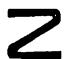
\includegraphics[keepaspectratio]{images/part002_ebb97593.jpg}}

\subsection{Extension of scalars in an integrally closed algebra}

PROPOSITION 19. Let \(k\) be a field, \(L\) a separable extension of \(k\) and \(R\) an integrally closed \(k\) -algebra. If the ring \(L \otimes_k R\) is an integral domain, it is integrally closed.

Let K be the field of fractions of R; as k is a field, \(L \otimes_{k} R\) is canonically identified with a sub-k-algebra of \(L \otimes_{k} K\) and L and R with sub-k-algebras of \(L \otimes_{k} R\) . Moreover, since an element \(s \neq 0\) of R is not a divisor of 0 in R, \(1 \otimes s\) is not a divisor of zero in \(L \otimes_{k} R\) since L is flat over k (Chapter I, §2, no. 3); identifying s with \(1 \otimes s\) , it is therefore seen that, if S = R - \{0\}, \(L \otimes_{k} K\) is identified with \(S^{-1}(L \otimes_{k} K)\) ; as \(L \otimes_{k} R\) is assumed to be an integral domain, \(L \otimes_{k} K\) is thus identified with a subring of the field of fractions \(\Omega\) of \(L \otimes_{k} R\) .

\begin{enumerate}
\def\labelenumi{(\arabic{enumi})}
\tightlist
\item
  Suppose that \(\mathbf{L}\) is a finite extension of \(k\) ; then \(\mathbf{L} \otimes_k \mathbf{K}\) is an algebra of finite rank over \(\mathbf{K}\) and by hypothesis has no divisor of 0; hence it is a field (Algebra, Chapter V, §2, no. 1, Proposition 1) and therefore it is in this case the field of fractions \(\Omega\) of \(\mathbf{L} \otimes_k \mathbf{R}\) . Let \((w_1, \ldots, w_n)\) be a basis of \(\mathbf{L}\) over \(k\) , which is therefore also a basis of \(\mathbf{L} \otimes_k \mathbf{K}\) over \(\mathbf{K}\) . There exists a basis \((w_1^*, \ldots, w_n^*)\) of \(\mathbf{L}\) such that \(\mathrm{Tr}_{\mathrm{L/k}}(w_i w_j^*) = \delta_{ij}\) (no. 6, Lemma 3); every \(z \in \mathbf{L} \otimes_k \mathbf{K}\) may be written uniquely \(z = \sum_{i=1}^{n} a_i w_i\) where \(a_i \in \mathbf{K}\) ; then
\end{enumerate}

\[
\operatorname{Tr} _ {(\mathrm{L} \otimes \mathrm{K}) / \mathrm{K}} (z w _ {j} ^ {*}) = \sum_ {i = 1} ^ {n} a _ {i} \operatorname{Tr} _ {(\mathrm{L} \otimes \mathrm{K}) / \mathrm{K}} (w _ {i} w _ {j} ^ {*})
\]

and as in L the traces \(\mathrm{Tr}_{(L\otimes K)/K}\) and \(\mathrm{Tr}_{L/K}\) coincide (Algebra, Chapter VIII, § 12, no. 2, formula (13)) finally \(\mathrm{Tr}_{(L\otimes K)/K}(zw_j^*) = a_j\) for \(1 \leqslant j \leqslant n\) . Note on the other hand that the elements of L are integral over \(k\) and hence also over R (no. 1, Corollary 1 to Proposition 2); therefore (no. 1, Proposition 5) \(\mathbf{L} \otimes_k \mathbf{R}\) is integral over R. This being so, suppose that \(z \in \mathbf{L} \otimes_k \mathbf{K}\) is integral over \(\mathbf{L} \otimes_k \mathbf{R}\) ; then \(z\) is also integral over R (no. 1, Proposition 6), hence so is \(zw_j^*\) and therefore also \(a_j = \mathrm{Tr}_{(L\otimes K)/K}(zw_j^*)\) for \(1 \leqslant j \leqslant n\) (no. 6, Corollary 2 to Proposition 17). As R is integrally closed, \(a_j \in \mathbf{R}\) for all \(j\) and hence \(z \in \mathbf{L} \otimes_k \mathbf{R}\) , which proves the proposition in this case.

\begin{enumerate}
\def\labelenumi{(\arabic{enumi})}
\setcounter{enumi}{1}
\tightlist
\item
  Suppose now that \(\mathbf{L}\) is a finitely generated separable extension of \(k\) ; then there exists a separating transcendence basis \((x_1, \ldots, x_d)\) of \(\mathbf{L}\) over \(k\) (Algebra, Chapter V, § 9, no. 3, Theorem 2); as \(\mathbf{L}\) and \(\mathbf{K}\) are algebraically disjoint over \(k\) in the field \(\Omega\) (Algebra, Chapter V, § 5, no. 4), the \(x_i\) are algebraically independent over \(\mathbf{K}\) ; hence \(\mathrm{R}[x_1, \ldots, x_d]\) is integrally closed (no. 3, Corollary 2 to Proposition 13). Let \(\mathbf{T}\) be the set of elements \(\neq 0\) of the ring \(\mathbf{A} = k[x_1, \ldots, x_d] \subset \mathbf{L}\) , so that the field \(k_1 = k(x_1, \ldots, x_d) \subset \mathbf{L}\) is equal to \(\mathbf{T}^{-1} k[x_1, \ldots, x_d]\) ; then
\end{enumerate}

\[
\begin{array}{r l} k _ {1} \otimes_ {k} \mathrm{R} & = (\mathrm{T} ^ {- 1} \mathrm{A}) \otimes_ {k} \mathrm{R} = \mathrm{T} ^ {- 1} \mathrm{A} \otimes_ {\mathrm{A}} (\mathrm{A} \otimes_ {k} \mathrm{R}) = \mathrm{T} ^ {- 1} (\mathrm{A} \otimes_ {k} \mathrm{R}) \\ & = \mathrm{T} ^ {- 1} \mathrm{R} [ x _ {1}, \dots , x _ {d} ] \end{array}
\]

by the associativity of the tensor product, hence this domain is integrally closed (no. 5, Corollary 1 to Proposition 16). But \(\mathbf{L} \otimes_k \mathbf{R}\) is identified with \(\mathbf{L} \otimes_{k_1} (k_1 \otimes_k \mathbf{R})\) and by definition \(\mathbf{L}\) is a finite separable extension of \(k_1\) ; it follows therefore from (1) that \(\mathbf{L} \otimes_k \mathbf{R}\) is integrally closed.

\begin{enumerate}
\def\labelenumi{(\arabic{enumi})}
\setcounter{enumi}{2}
\tightlist
\item
  General case. If z is an element of \(\Omega\) which is integral over \(L \otimes_{k} R\) , it satisfies a relation of the form \(z^{m} + b_{1}z^{m-1} + \cdots + b_{m} = 0\) , where the \(b_{i}\) belong to \(L \otimes_{k} R\) ; then there exists a finitely generated sub-extension \(L'\) of L over k such that the \(b_{i}\) belong to \(L' \otimes_{k} R\) for \(1 \leqslant i \leqslant m\) and z to \(L' \otimes_{k} K\) . Then it follows from (2) that \(z \in L' \otimes_{k} R\) and hence \(L \otimes_{k} R\) is integrally closed.
\end{enumerate}

* Let V be an affine irreducible algebraic variety, k a defining field of V and R the ring of functions regular on V defined over k; if R is integrally closed, V is called normal over k; Proposition 19 shows that, if V is normal over k, it remains normal over every separable extension L of k. *

COROLLARY. Let \(k\) be a field and \(\mathbf{R}\) and \(\mathbf{S}\) two integrally closed \(k\) -algebras. Suppose that the ring \(\mathbf{R} \otimes_k \mathbf{S}\) is an integral domain and that the fields of fractions \(\mathbf{K}\) and \(\mathbf{L}\) of \(\mathbf{R}\) and \(\mathbf{S}\) respectively are separable over \(k\) . Then the ring \(\mathbf{R} \otimes_k \mathbf{S}\) is an integrally closed domain.

As R and S are identified with subalgebras of \(R \otimes_{k} S\) , K and L are identified with subfields of the field of fractions \(\Omega\) of \(R \otimes_{k} S\) which are linearly disjoint over k (Algebra, Chapter V, §2, no. 3, Proposition 5). It then follows from Proposition 19 that \(R \otimes_{k} L\) and \(K \otimes_{k} S\) are integrally closed domains; as their intersection is \(R \otimes_{k} S\) (Chapter I, §2, no. 6, Proposition 7), \(R \otimes_{k} S\) is an integrally closed domain (no. 2, Corollary to Proposition 8).

* Given two irreducible affine varieties V, W defined over k, their product \(V \times W\) is an affine variety and the ring of functions regular on \(V \times W\) is identified with the tensor product over k of the ring of functions regular on V and the ring of functions regular on W. The Corollary to Proposition 19 shows that, if V and W are normal over k, then \(V \times W\) is normal over k. *

\subsection{Integers over a graded ring}

All the graduations considered in this no. are of type Z; if A is a graded ring and \(i \in Z\) , \(A_{i}\) denotes the set of homogeneous elements of degree i of the ring A.

Let A be a graded ring and B a graded A-algebra. Let x be a homogeneous element of B which is integral over A; then there is a relation

\[
x ^ {n} + a _ {1} x ^ {n - 1} + \dots + a _ {n} = 0 \quad \text { where } \quad a _ {i} \in A \quad \text { for } \quad 1 \leqslant i \leqslant n.\tag{3}
\]

Let \(m = \deg(x)\) and let \(a_i'\) be the homogeneous component of degree \(mi\) of \(a_i\) ( \(1 \leqslant i \leqslant n\) ); then obviously

\[
x ^ {n} + a _ {1} ^ {\prime} x ^ {n - 1} + \dots + a _ {n} ^ {\prime} = 0\tag{4}
\]

in other words x satisfies an equation of integral dependence with homogeneous coefficients.

Let \(\mathbf{A}[\mathbf{X},\mathbf{X}^{-1}]\) denote the ring of fractions \(\mathbf{S}^{-1}\mathbf{A}[\mathbf{X}]\) of the polynomial ring \(\mathbf{A}[\mathbf{X}]\) in one indeterminate, \(\mathbf{S}\) being the multiplicative subset of \(\mathbf{A}[\mathbf{X}]\) consisting of the powers \(\mathbf{X}^n\) of \(\mathbf{X}\) ( \(n\geqslant 0\) ); as \(\mathbf{X}\) is not a divisor of 0 in \(\mathbf{A}[\mathbf{X}]\) it is immediate that the \(\mathbf{X}^i\) ( \(i\in \mathbf{Z}\) ) form a basis over \(\mathbf{A}\) of the A-module \(\mathbf{A}[\mathbf{X},\mathbf{X}^{-1}]\) . For every element \(a\in \mathbf{A}\) with homogeneous components \(a_{i}\) ( \(i\in \mathbf{Z}\) ), we write

\iffalse
\begin{description}
\tightlist
\item[\$\$]
j \_ \{\mathbf {A}\} (a) = \sum\_ \{i \in \mathbf {Z}\} a \_ \{i\} \mathbf {X} \^{} \{i\} \in \mathrm{A} {[} \mathbf {X}, \mathbf {X} \^{} \{- 1\} {]}\tag{5} \$\$
\end{description}
\fi

\[
:j_{A}(a) = \sum_{i \in \mathbf{Z}} a_{i} \mathbf{X}^{i} \in \mathbf{A}[\mathbf{X},\mathbf{X}^{-1}]\tag{5}
\]

it is immediate that \(j_{A}: A \to A[X, X^{-1}]\) is an injective ring homomorphism.

PROPOSITION 20. Let \(\mathbf{A} = \bigoplus_{i\in \mathbf{Z}}\mathbf{A}_i\) be a graded ring and \(\mathbf{B}\) a (commutative) graded A-algebra. The set \(\mathbf{A}'\) of elements of \(\mathbf{B}\) integral over \(\mathbf{A}\) is a graded subalgebra of \(\mathbf{B}\) . If \(\mathbf{A}_i = 0\) for \(i < 0\) and \(\mathbf{B}\) is a reduced ring, then \(\mathbf{A}_i' = 0\) for \(i < 0\) .

If \(\mathbf{A}_i = 0\) for \(i < 0\) and \(\mathbf{B}\) is a reduced ring, then \(\mathbf{A}_i' = 0\) for \(i < 0\) . The diagram

\pandocbounded{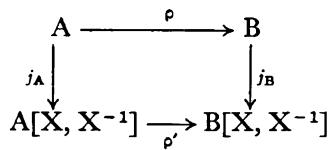
\includegraphics[keepaspectratio]{images/part002_18d5f867.jpg}}

(where \(\rho\) is the homomorphism defining the A-algebra structure on B and \(\rho'\) the homomorphism canonically derived from it) is commutative, as is immediately verified from the definition (5). Let \(x\) be an element of B integral over A; then \(j_{\mathrm{B}}(x)\) is integral over \(\mathbf{A}[\mathbf{X}, \mathbf{X}^{-1}]\) (no. 1, Proposition 2) and it therefore follows from no. 5, Proposition 16 that there exists an integer \(m > 0\) such that \(\mathbf{X}^m j_{\mathrm{B}}(x)\) is an element of \(\mathbf{B}[\mathbf{X}]\) integral over \(\mathbf{A}[\mathbf{X}]\). We then deduce from no. 3, Proposition 12 that the coefficients of the polynomial \(\mathbf{X}^m j_{\mathrm{B}}(x)\) are integral over A; as these coefficients are by definition the homogeneous components of \(x\) , it is seen that these are integral over A, which proves that \(\mathbf{A}'\) is a graded subalgebra of B.

Suppose now that \(x \in \mathbf{A}_i'\) where \(i < 0\) ; the remark at the beginning of this no. shows that \(x\) satisfies an equation of the form (4) where \(a_k' \in \mathbf{A}_{ki}\) for \(1 \leqslant k \leqslant n\) . If \(\mathbf{A}_j = 0\) for \(j < 0\) , then \(x^n = 0\) and if \(B\) is a reduced ring we conclude that \(x = 0\) and hence \(\mathbf{A}_i' = 0\) for all \(i < 0\) in this case.

Recall (Chapter II, § 2, no. 9) that, if \(\mathbf{A} = \bigoplus_{i\in \mathbf{Z}}\mathbf{A}_i\) is a graded ring and S is a multiplicative subset of A consisting of homogeneous elements, a graded ring structure is defined on \(\mathrm{S}^{-1}\mathrm{A}\) by taking the set \((\mathrm{S}^{-1}\mathrm{A})_i\) of homogeneous elements of degree \(i\) to be the set of elements of the form \(a / s\) , where \(a\in \mathbf{A}\) and \(s\in \mathbf{S}\) are homogeneous and such that \(\deg (a) - \deg (s) = i\) .

LEMMA 4. Let \(\mathbf{A} = \bigoplus_{i\in \mathbf{Z}}\mathbf{A}_i\) be a graded integral domain and S the set of homogeneous elements \(\neq 0\) of A.

\begin{enumerate}
\def\labelenumi{(\roman{enumi})}
\item
  Every homogeneous element \(\neq 0\) of \(\mathbf{S}^{-1}\mathbf{A}\) is invertible, the ring \(\mathbf{K}_0 = (\mathbf{S}^{-1}\mathbf{A})_0\) is a field and the set of \(i\in \mathbf{Z}\) such that \((\mathrm{S}^{-1}\mathrm{A})_i\neq 0\) is a subgroup \(q\mathbf{Z}\) of \(\mathbf{Z}\) (where \(q\geqslant 0\) ).
\item
  Suppose that \(q \geqslant 1\) and let \(t\) be a non-zero element of \((\mathbf{S}^{-1}\mathbf{A})_q\) . Then the \(\mathbf{K}_0\) -homomorphism \(f\) of the polynomial ring \(\mathbf{K}_0[\mathbf{X}]\) to \(\mathbf{S}^{-1}\mathbf{A}\) which maps \(\mathbf{X}\) to \(t\) extends to an isomorphism of \(\mathbf{K}_0[\mathbf{X}, \mathbf{X}^{-1}]\) onto \(\mathbf{S}^{-1}\mathbf{A}\) and \(\mathbf{S}^{-1}\mathbf{A}\) is integrally closed.
\end{enumerate}

The assertions in (i) follow immediately from the definitions and the hypothesis that A is an integral domain, for if \(a/s\) and \(a'/s'\) are two homogeneous elements \(\neq 0\) of \(\mathrm{S}^{-1}\mathrm{A}\) of degrees \(i\) and \(i'\) , \(aa'/ss'\) is a homogeneous element \(\neq 0\) and of degree \(i+i'\) . To show (ii), we note that since \(t\) is invertible in \(\mathrm{S}^{-1}\mathrm{A}\) the homomorphism \(f\) extends in a unique way to a homomorphism \(\bar{f}: \mathrm{K}_0[\mathrm{X}, \mathrm{X}^{-1}] \to \mathrm{S}^{-1}\mathrm{A}\) and necessarily \(\bar{f}(\mathrm{X}^{-1}) = t^{-1}\) . On the other hand, by definition of \(q\) , every homogeneous element \(\neq 0\) of \(\mathrm{S}^{-1}\mathrm{A}\) is of degree \(qn\) ( \(n \in \mathbf{Z}\) ) and hence can be written uniquely in the form \(\lambda t^n\) where \(\lambda \in \mathrm{K}_0\) (since \(\mathrm{S}^{-1}\mathrm{A}\) is an integral domain); hence \(\bar{f}\) is bijective. Finally, we know that \(\mathrm{K}_0[\mathrm{X}]\) is integrally closed (no. 3, Proposition 10) and hence so is \(\mathrm{K}_0[\mathrm{X}, \mathrm{X}^{-1}]\) (no. 5, Corollary 1 to Proposition 16), which completes the proof of the Lemma.

PROPOSITION 21. Let \(\mathbf{A} = \bigoplus_{i\in \mathbf{Z}}\mathbf{A}_i\) be a graded integral domain and S the set of homogeneous elements \(\neq 0\) of A. The integral closure \(\mathbf{A}'\) of A is then a graded subring of \(\mathbf{S}^{-1}\mathbf{A}\) . If further \(\mathbf{A}_i = 0\) for \(i < 0\) , then \(\mathbf{A}_i' = 0\) for \(i < 0\) .

If \(A = A_{0}\) , the proposition is trivial. Otherwise we may apply Lemma 4; the ring \(S^{-1}A\) is an integrally closed domain and therefore \(A' \subset S^{-1}A\) ; as \(S^{-1}A\) is graded, so is \(A'\) by Proposition 20; the latter assertion also follows from Proposition 20.

COROLLARY 1. With the hypotheses and notation of Proposition 21, if every homogeneous element of \(\mathbf{S}^{-1}\mathbf{A}\) which is integral over \(\mathbf{A}\) belongs to \(\mathbf{A}\) , then \(\mathbf{A}\) is integrally closed.

Then \(\mathbf{A}_i' \subset \mathbf{A}\) for all \(i \in \mathbf{Z}\) and hence \(\mathbf{A}' = \mathbf{A}\) .

COROLLARY 2. If \(\mathbf{A} = \bigoplus_{i\in \mathbf{Z}}\mathbf{A}_i\) is an integrally closed graded domain, the domain \(\mathbf{A}_0\) is integrally closed.

The field of fractions \(\mathbf{K}_0\) of \(\mathbf{A}_0\) is identified (in the notation of Proposition 21)

with a subring of the ring of homogeneous elements of degree 0 of \(S^{-1}A\) ; every element of \(K_{0}\) integral over \(A_{0}\) (and a fortiori over A) belongs therefore by hypothesis to \(A_{0}\) .

COROLLARY 3. Let \(\mathbf{A} = \bigoplus_{i\in \mathbf{Z}}\mathbf{A}_i\) be an integrally closed graded domain. Then, for every integer \(d > 0\) , the ring \(\mathbf{A}^{(d)}\) (Chapter III, §1, no. 3) is an integrally closed domain.

Let U be the set of homogeneous elements \(\neq0\) of \(A^{(d)}\) and let x be a homogeneous element of \(U^{-1}A^{(d)}\) integral over \(A^{(d)}\) and hence over A; as \(x\in S^{-1}A\) , x belongs to A by hypothesis; as its degree is divisible by d, it belongs to \(A^{(d)}\) and it then follows from Corollary 1 that \(A^{(d)}\) is integrally closed.

\subsection{Application: invariants of a group of automorphisms of an algebra}

Given a ring K, a K-algebra A and a group G, we shall say that G operates on A if: (1) the set A has group of operators G (Algebra, Chapter I, § 7, no. 2); (2) for all \(\sigma \in G\) , the mapping \(x \mapsto \sigma \cdot x\) is an endomorphism of the K-algebra A (and therefore an automorphism since it is bijective (loc. cit.)). We shall denote by \(A^{G}\) , the set of elements of A which are invariant under G; clearly it is a sub-K-algebra of A.

We shall say that \(\mathcal{G}\) is a locally finite group of operators on A if every orbit of \(\mathcal{G}\) in A (Algebra, Chapter I, Corrections to Fascicule IV) is finite.

PROPOSITION 22. Let A be a (commutative) K-algebra and G a locally finite group of operators on A. Then A is integral over the subalgebra \(\mathbf{A}^{\mathcal{G}}\) .

For all \(x \in \mathbf{A}\) , let \(x_{i} (1 \leqslant i \leqslant n)\) be the distinct elements of the orbit of \(x\) under \(\mathcal{G}\) ; for all \(\sigma \in \mathcal{G}\) , there exists a permutation \(\pi_{\sigma}\) of the set \(\{1, 2, \ldots, n\}\) such that \(\sigma. x_{i} = x_{\pi_{\sigma}(i)}\) for \(1 \leqslant i \leqslant n\) ; therefore the elementary symmetric functions of the \(x_{i}\) are elements of \(\mathbf{A}\) which are invariant under \(\mathcal{G}\) , in other

words elements of \(\mathbf{A}^{\mathcal{G}}\) . As \(x\) is a root of the monic polynomial \(\prod_{i=1}^{n} (\mathbf{X} - x_i)\) and the coefficients of this polynomial belong to \(\mathbf{A}^{\mathcal{G}}\) , \(x\) is integral over \(\mathbf{A}^{\mathcal{G}}\) .

THEOREM 2. Let A be a finitely generated K-algebra and G a locally finite group of operators on A. Then A is a finitely generated \(\mathbf{A}^{\mathcal{G}}\)-module; if further K is Noetherian, \(A^{G}\) is a finitely generated K-algebra.

Let \((a_{j})_{1\leqslant j\leqslant m}\) be a system of generators of the K-algebra A; as a fortiori \(\mathbf{A} = \mathbf{A}^{\mathcal{G}}[a_1,\ldots ,a_m]\) and the \(a_{j}\) are integral over \(\mathbf{A}^{\mathcal{G}}\) by Proposition 22, the first assertion follows from no. 1, Proposition 4. The second is a consequence of the following lemma:

LEMMA 5. Let K be a Noetherian ring, B a finitely generated K-algebra and C a sub-K-algebra of B such that B is integral over C. Then C is a finitely generated K-algebra.

Let \((x_{i})_{1\leqslant i\leqslant n}\) be a finite system of generators of the K-algebra B. For all \(i\) , there exists by hypothesis a monic polynomial \(\mathbf{P}_i\in \mathbf{C}[\mathbf{X}]\) such that \(\mathrm{P_i}(x_i) = 0\) . Let \(\mathbf{C}'\) be the sub-K-algebra of C generated by the coefficients of the \(\mathbf{P}_i\) ( \(1\leqslant i\leqslant n\) ); clearly the \(x_{i}\) are integral over \(\mathbf{C}'\) and \(\mathbf{B} = \mathbf{C}'[x_1,\dots,x_n]\) ; hence B is a finitely generated \(\mathbf{C}'\) -module (no. 1, Proposition 4). On the other hand \(\mathbf{C}'\) is a Noetherian ring (Chapter III, §2, no. 10, Corollary 3 to Theorem 2); hence C is a finitely generated \(\mathbf{C}'\) -module, which proves that C is a finitely generated K-algebra.

Remark. The set of \(\sigma \in \mathcal{G}\) such that \(\sigma a_{j} = a_{j}\) for \(1 \leqslant j \leqslant m\) obviously leaves invariant every element of A. The normal subgroup \(\mathcal{H}\) of \(\mathcal{G}\) leaving invariant every element of A is therefore of finite index in \(\mathcal{G}\) and A may be considered as having a finite group of operators \(\mathcal{G}/\mathcal{H}\) ; obviously \(\mathrm{A}^{\mathcal{G}/\mathcal{H}} = \mathrm{A}^{\mathcal{G}}\) .

Let S be a multiplicative subset of a ring A and G a group operating on A and for which S is stable; then, for all \(\sigma\in G\) , there exists a unique endomorphism \(z\mapsto\sigma.z\) of the ring \(S^{-1}A\) such that \(\sigma.(a/1)=(\sigma.a)/1\) for all \(a\in A\) ; it is given by the formula \(\sigma.(a/s)=(\sigma.a)/( \sigma.s)\) for \(a\in A\) and \(s\in S\) (Chapter II, §2, no. 1, Proposition 2); if \(\tau\) is another element of G, clearly \(\sigma.(\tau.z)=(\sigma\tau).z\) for all \(z\in S^{-1}A\) and hence the group G operates on the ring \(S^{-1}A\) .

PROPOSITION 23. Let A be a K-algebra, \(\mathcal{G}\) a locally finite group of operators on A, S a multiplicative subset of A stable under \(\mathcal{G}\) and \(\mathrm{S}^{\mathcal{G}}\) the set \(\mathrm{S} \cap \mathrm{A}^{\mathcal{G}}\) . Then the canonical mapping of \((\mathrm{S}^{\mathcal{G}})^{-1}\mathrm{A}\) to \(\mathrm{S}^{-1}\mathrm{A}\) (Chapter II, § 2, no. 1, Corollary 2 to Proposition 2) is an isomorphism which maps \((\mathrm{S}^{\mathcal{G}})^{-1}\mathrm{A}^{\mathcal{G}}\) to \((\mathrm{S}^{-1}\mathrm{A})^{\mathcal{G}}\) .

For all \(s \in S\) , let \(s, s_1, \ldots, s_q\) be the distinct elements of the orbit of \(s\) under \(\mathcal{G}\) ; as \(ss_1 \ldots s_q \in S^{\mathcal{G}}\) , the first assertion follows from Chapter II, § 2, no. 3, Proposition 8. Identifying canonically \((S^{\mathcal{G}})^{-1}A\) with \(S^{-1}A\) , clearly every element of \((S^{\mathcal{G}})^{-1}A^{\mathcal{G}}\) is invariant under \(\mathcal{G}\) . Conversely, let \(a/t\) be an element of \((S^{\mathcal{G}})^{-1}A\) which is invariant under \(\mathcal{G}\) ( \(a \in A\) , \(t \in S^{\mathcal{G}}\) ); if \(a_j\) ( \(1 \leqslant j \leqslant m\) ) are the distinct elements of the orbit of \(a\) under \(\mathcal{G}\) , then \(a_j/t = a/t\) for \(1 \leqslant j \leqslant m\) and therefore there exists \(s \in S^{\mathcal{G}}\) such that \(s(a_j - a) = 0\) for \(1 \leqslant j \leqslant m\) ; in other words, \(sa\) is invariant under \(\mathcal{G}\) and, as \(a/t = (sa)/(st)\) , certainly \(a/t \in (S^{\mathcal{G}})^{-1}A^{\mathcal{G}}\) .

COROLLARY. Let A be an integral domain, K its field of fractions and G a locally finite group of operators on A. Then G operates on K and \(K^{G}\) is the field of fractions of \(A^{G}\) .

A - \{0\} is stable under G.

\section{THE LIFT OF PRIME IDEALS}

\subsection{The first existence theorem}

DEFINITION 1. Let A, A' be two rings and h: A → A' a ring homomorphism. An ideal a' of A' is said to lie above an ideal a of A if \iffalse h\^{}\{-1\}(a')\fi\(a = h^{-1}(a')\).

To say that a prime ideal \(\mathfrak{p}'\) of \(\mathbf{A}'\) lies above an ideal \(\mathfrak{p}\) of \(\mathbf{A}\) therefore means that \(\mathfrak{p}\) is the image of \(\mathfrak{p}'\) under the continuous mapping \(^a h\) : \(\operatorname{Spec}(\mathbf{A}') \to \operatorname{Spec}(\mathbf{A})\) associated with \(h\) (Chapter II, § 4, no. 3).

Note that for there to exist an ideal of \(\mathbf{A}'\) lying above the ideal (0) of \(\mathbf{A}\) , it is necessary and sufficient that \(h: \mathbf{A} \to \mathbf{A}'\) be injective.

Let \(\mathfrak{a}\) be an ideal of \(\mathbf{A}\) ; by taking quotients the homomorphism \(h\) gives a homomorphism \(h_1: \mathbf{A} / \mathfrak{a} \to \mathbf{A}' / \mathfrak{a}'\) ; to say that \(\mathfrak{a}'\) is an ideal of \(\mathbf{A}'\) lying above \(\mathfrak{a}\) is equivalent to saying that \(\mathfrak{a}\mathbf{A}' \subset \mathfrak{a}'\) and that \(\mathfrak{a}' / \mathfrak{a}\mathbf{A}'\) is an ideal of \(\mathbf{A}' / \mathfrak{a}\mathbf{A}'\) lying above (0).

LEMMA 1. Let \(h: \mathbf{A} \to \mathbf{A}'\) be a ring homomorphism, \(\mathbf{S}\) a multiplicative subset of \(\mathbf{A}\) , \(i = i_{\mathbf{A}}^{\mathbf{S}}: \mathbf{A} \to \mathbf{S}^{-1}\mathbf{A}\) , \(i' = i_{\mathbf{A}'}^{h(\mathbf{S})}: \mathbf{A}' \to \mathbf{S}^{-1}\mathbf{A}' = (h(\mathbf{S}))^{-1}\mathbf{A}'\) the canonical homomorphisms and \(h_1 = \mathbf{S}^{-1}h: \mathbf{S}^{-1}\mathbf{A} \to \mathbf{S}^{-1}\mathbf{A}'\) , so that there is a commutative diagram

\pandocbounded{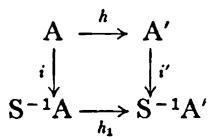
\includegraphics[keepaspectratio]{images/part002_a0a90333.jpg}}

Let \(\mathfrak{p}\) be a prime ideal of \(\mathbf{A}\) such that \(\mathfrak{p} \cap \mathbf{S} = \varnothing\) . Then \(\mathfrak{a}' \mapsto \mathbf{S}^{-1}\mathfrak{a}'\) is a surjective mapping of the set \(\mathcal{F}\) of ideals of \(\mathbf{A}'\) lying above \(\mathfrak{p}\) onto the set \(\mathcal{F}_1\) of ideals of \(\mathbf{S}^{-1}\mathbf{A}'\) lying above \(\mathbf{S}^{-1}\mathfrak{p}\) and the mapping \(\mathfrak{a}_1' \mapsto i'^{-1}(\mathfrak{a}_1')\) is a bijection of \(\mathcal{F}_1\) onto the set of ideals belonging to \(\mathcal{F}\) and is saturated with respect to \(h(S)\) ; in particular \(\mathfrak{p}' \mapsto \mathbf{S}^{-1}\mathfrak{p}'\) is a bijection of the set of prime ideals of \(\mathbf{A}'\) lying above \(\mathfrak{p}\) onto the set of prime ideals of \(\mathbf{S}^{-1}\mathbf{A}'\) lying above \(\mathbf{S}^{-1}\mathfrak{p}\) .

We know that \(\mathbf{S}^{-1}\mathfrak{p}\) is a prime ideal of \(\mathbf{S}^{-1}\mathbf{A}\) and that \(i^{-1}(\mathbf{S}^{-1}\mathfrak{p}) = \mathfrak{p}\) (Chapter II, § 2, no. 5, Proposition 11); if there exists an ideal \(\mathfrak{b}'\) of \(\mathbf{S}^{-1}\mathbf{A}'\) lying above \(\mathbf{S}^{-1}\mathfrak{p}\) , then \(h(i'^{-1}(\mathfrak{b}')) = i^{-1}(h_1(\mathfrak{b}')) = \mathfrak{p}\) ; as \(\mathbf{S}^{-1}.i'^{-1}(\mathfrak{b}') = \mathfrak{b}'\) (loc. cit.), this already shows that the image of \(\mathcal{F}\) under the mapping \(\mathfrak{a}'\mapsto\mathrm{S}^{-1}\mathfrak{a}'\) contains \(\mathcal{F}_{1}\) . On the other hand, if \(\mathfrak{a}'\in\mathcal{F}\) , \(a\in\mathbf{A}\) and \(s\in\mathbf{S}\) , there are the following equivalences

\[
\begin{array}{l} h _ {1} (a / s) \in \mathrm{S} ^ {- 1} \mathfrak {a} ^ {\prime} \Leftrightarrow h (a) / h (s) \in \mathrm{S} ^ {- 1} \mathfrak {a} ^ {\prime} \\ \Leftrightarrow \text { there   exists } t \in \mathrm{S} \text { such   that } h (t) h (a) \in \mathfrak {a} ^ {\prime} \\ \Leftrightarrow \text { there   exists } t \in \mathrm{S} \text { such   that } t a \in \mathfrak {p} \\ \Leftrightarrow a / s \in \mathrm{S} ^ {- 1} \mathfrak {p}. \end{array}
\]

Hence \(h_1^{-1}(\mathbf{S}^{-1}\mathfrak{a}') = \mathbf{S}^{-1}\mathfrak{p}\) , which completes the proof that the image of \(\mathcal{F}\) under the mapping \(\mathfrak{a}' \mapsto \mathbf{S}^{-1}\mathfrak{a}'\) is equal to \(\mathcal{F}_1\) ; the other assertions follow from Chapter II, § 2, no. 5, Proposition 11.

PROPOSITION 1. Let \(h: \mathbf{A} \to \mathbf{A}'\) be a ring homomorphism such that \(\mathbf{A}'\) is integral over \(\mathbf{A}\) , \(\mathfrak{p}'\) a prime ideal of \(\mathbf{A}'\) and \(\mathfrak{p} = h^{-1}(\mathfrak{p}')\) . For \(\mathfrak{p}\) to be maximal, it is necessary and sufficient that \(\mathfrak{p}'\) be so.

Let us write \(\mathrm{B} = \mathrm{A} / \mathfrak{p}\) , \(\mathrm{B}' = \mathrm{A}' / \mathfrak{p}'\) and let \(h_1 \colon \mathrm{B} \to \mathrm{B}'\) be the homomorphism derived from \(h\) by taking quotients; \(\mathrm{B}\) and \(\mathrm{B}'\) are integral domains and \(\mathrm{B}'\) is integral over \(\mathrm{B}\) (§ 1, no. 1, Proposition 2). To say that \(\mathfrak{p}\) (resp. \(\mathfrak{p}'\) ) is maximal means that \(\mathrm{B}\) (resp. \(\mathrm{B}'\) ) is a field. The proposition then follows from the following lemma:

LEMMA 2. Let B be an integral domain and A a subring of B such that B is integral over A. For B to be a field, it is necessary and sufficient that A be a field.

If A is a field, then, for all \(y \neq 0\) in B, A[y] is by hypothesis ( \(\S 1\) , Theorem 1) a finitely generated A-module; as A[y] is an integral domain, it is a field (Algebra, Chapter V, \(\S 2\) , no. 1, Proposition 1) and a fortiori y is invertible in B and hence B is a field. Conversely, suppose that B is a field and let \(z \neq 0\) in A; as \(z^{-1} \in B\) , \(z^{-1}\) is integral over A, in other words there is an equation of integral dependence

\[
z ^ {- n} + a _ {1} z ^ {- (n - 1)} + \dots + a _ {n} = 0
\]

where the \(a_{i} \in \mathbf{A}\) ; now this relation shows that

\[
- z ^ {- 1} = a _ {1} + a _ {2} z + \dots + a _ {n} z ^ {n - 1} \in A,
\]

hence A is certainly a field.

COROLLARY 1. Let \(h: \mathbf{A} \to \mathbf{A}'\) be a ring homomorphism such that \(\mathbf{A}'\) is integral over \(\mathbf{A}\) , \(\mathfrak{p}\) a prime ideal of \(\mathbf{A}\) and \(\mathfrak{p}'\) and \(\mathfrak{a}'\) two ideals of \(\mathbf{A}'\) lying above \(\mathfrak{p}\) such that \(\mathfrak{p}' \subset \mathfrak{a}'\) . If \(\mathfrak{p}'\) is prime, then \(\mathfrak{a}' = \mathfrak{p}'\) .

Let us write \(S = A - p\) ; then \(S^{-1}A'\) is integral over \(S^{-1}A\) (§ 1, no. 5, Proposition

16), \(S^{-1}p\) is a maximal ideal of \(S^{-1}A\) (Chapter II, §2, no. 5, Proposition 11), \(S^{-1}a'\) and \(S^{-1}p'\) are ideals of \(S^{-1}A'\) lying above \(S^{-1}p\) (Lemma 1) and \(S^{-1}a' \supseteq S^{-1}p'\) . As \(S^{-1}p'\) is prime, it is maximal by Proposition 1 and hence \(S^{-1}p' = S^{-1}a'\) ; therefore \(a'\) is contained in the saturation of \(p'\) with respect to \(h(S)\) , which is equal to \(p'\) (Chapter II, §2, no. 5, Proposition 11).

COROLLARY 2. Let A' be an integral domain, A a subring of A' such that A' is integral over A and f a homomorphism from A' to a ring B. If the restriction of f to A is injective, f is injective.

If \(a'\) is the kernel of f, the hypothesis means that \(a' \cap A = (0)\) ; as \(A'\) is an integral domain, Corollary 1 may be applied taking p and \(p'\) to be the ideal (0) of A and the ideal (0) of \(A'\) respectively, whence \(a' = (0)\) .

COROLLARY 3. Let \(h: \mathbf{A} \to \mathbf{A}'\) be a ring homomorphism such that \(\mathbf{A}'\) is integral over \(\mathbf{A}\) and \(\mathfrak{m}\) a maximal ideal of \(\mathbf{A}\) and suppose that there are in \(\mathbf{A}'\) only a finite number of distinct maximal ideals \(\mathfrak{m}_j' (1 \leqslant j \leqslant n)\) lying above \(\mathfrak{m}\) . Let \(\mathfrak{q}_j'\) be the saturation of \(\mathfrak{mA}'\) with respect to \(\mathfrak{m}_j'\) (Chapter II, § 2, no. 4). Then:

\begin{enumerate}
\def\labelenumi{(\roman{enumi})}
\item
  In the ring \(\mathbf{A}' / \mathfrak{q}_j'\) the divisors of zero are the elements of \(\mathfrak{m}_j' / \mathfrak{q}_j'\) and they are nilpotent ( \(1 \leqslant j \leqslant n\) ).
\item
  \(mA' = \bigcap_{j} q_{j}' = \prod_{j} q_{j}'\) .
\item
  The canonical homomorphism \(\mathbf{A}' / \mathfrak{m}\mathbf{A}' \to \prod_j (\mathbf{A}' / \mathfrak{q}_j')\) is bijective.
\end{enumerate}

For a prime ideal of A' to contain mA', it is necessary and sufficient that its inverse image under h contain m and hence that it lie above m, since m is maximal in A; the \(m_{j}'\) are therefore the only prime ideals of A' containing mA' (Proposition 1) and therefore \(r' = \bigcap_{j} m_{j}'\) is the radical of mA' (Chapter II, §2, no. 6, Corollary 1 to Proposition 13). By definition of \(q_{j}'\) , the class mod. \(q_{j}'\) of an element of \(\mathbf{A}' - \mathfrak{m}_{j}'\) is not a divisor of 0 in \(A'/q_{j}'\); on the other hand, as the \(m_{j}'\) are distinct maximal ideals, for every index j there exists an element \(a_{j}'\) belonging to \(\bigcap_{i \neq j} m_{i}'\) and not to \(m_{j}'\) (Chapter II, §1, no. 1, Proposition 4); then, for all \(x \in m_{j}'\) , \(a_{j}'x \in r'\) , hence the class mod. \(q_{j}'\) of \(a_{j}'x\) is nilpotent and, as that of \(a_{j}'\) is not a divisor of 0, we conclude that the class of x is nilpotent; in other words \(m_{j}'\) is the radical of \(q_{j}'\) , which proves (i). It follows that the \(q_{j}'\) are relatively prime in pairs (Chapter II, §1, no. 1, Proposition 3); (iii) will therefore be a consequence of (ii), taking account of Chapter II, §1, no. 2, Proposition 5. To establish (ii), we note that in the ring A'/mA' the \(m_{j}'/mA'\) are the only maximal ideals and \(q_{j}'/mA'\) is the saturation of (0) with respect to \(m_{j}'/mA'\) (Chapter II, §2, no. 4); we may therefore restrict our attention to the case mA' = (0); the assertion of (ii) then follows from Chapter II, §3, no. 3, Corollary 2 to Theorem 1.

Remark (1) If \(\mathbf{A}'\) is Noetherian, it follows from (i) and (ii) that \((\mathfrak{q}_j')_{1 \leqslant j \leqslant n}\) is the unique primary decomposition of \(\mathfrak{mA}'\) (Chapter IV, § 2, no. 3).

THEOREM 1. Let \(h: \mathbf{A} \to \mathbf{A}'\) be an injective ring homomorphism such that \(\mathbf{A}'\) is integral over \(\mathbf{A}\) and \(\mathfrak{p}\) a prime ideal of \(\mathbf{A}\) . There exists a prime ideal \(\mathfrak{p}'\) of \(\mathbf{A}'\) lying above \(\mathfrak{p}\) .

Suppose first that A is a local ring and p the maximal ideal of A; then, for every maximal ideal \(m'\) of \(A'\) , \(\bar{h}^{-1}(m')\) is a maximal ideal of A (Proposition 1) and hence equal to p, which proves the theorem in this case (since \(A'\) contains A by hypothesis and is therefore not reduced to 0). In the general case, let us write \(S = A - p\) ; then \(S^{-1}A\) is a local ring whose maximal ideal is \(S^{-1}p\) (Chapter II, §2, no. 5, Proposition 11), \(S^{-1}h: S^{-1}A \to S^{-1}A'\) is injective (Chapter II, §2, no. 4, Theorem 1) and \(S^{-1}A'\) is integral over \(S^{-1}A\) (§1, no. 5, Proposition 16); then there exists a prime ideal \(q'\) of \(S^{-1}A'\) lying above \(S^{-1}p\) and we know that \(q' = S^{-1}p'\) , where \(p'\) is a prime ideal of \(A'\) lying above p (Lemma 1).

If \(h: \mathbf{A} \to \mathbf{A}'\) is not injective, Theorem 1 is no longer necessarily true, as the example of the homomorphism \(\mathbf{Z} \to \mathbf{Z}/n\mathbf{Z}\) ( \(n > 1\) ) shows. However Theorem 1 can be applied to the canonical injection \(h(\mathbf{A}) \to \mathbf{A}'\) ; in other words, the statement of Theorem 1 is true for prime ideals \(\mathfrak{p}\) containing \(\operatorname{Ker}(h)\) .

COROLLARY 1. With the hypotheses and notation of Theorem 1, \(h^{-1}(pA') = p\) .

\(\mathfrak{pA}' \subset \mathfrak{p}'\) and \(\overline{h}(\mathfrak{p}') = \mathfrak{p}\) .

COROLLARY 2. Let \(h: \mathbf{A} \to \mathbf{A}'\) be a ring homomorphism such that \(\mathbf{A}'\) is integral over \(\mathbf{A}\) , \(\mathfrak{a}\) and \(\mathfrak{p}\) two ideals of \(\mathbf{A}\) such that \(\mathfrak{a} \subset \mathfrak{p}\) and \(\mathfrak{a}'\) an ideal of \(\mathbf{A}'\) lying above \(\mathfrak{a}\) . Suppose that \(\mathfrak{p}\) is prime. Then there exists a prime ideal \(\mathfrak{p}'\) of \(\mathbf{A}'\) lying above \(\mathfrak{p}\) and containing \(\mathfrak{a}'\) .

If \(h_1 \colon \mathbf{A} / \mathfrak{a} \to \mathbf{A}' / \mathfrak{a}'\) is the homomorphism derived from \(h\) by taking quotients, \(h_1\) is injective by hypothesis and \(\mathbf{A}' / \mathfrak{a}'\) is integral over \(\mathbf{A} / \mathfrak{a}\) (§ 1, no. 1, Proposition 2); then there exists a prime ideal \(\mathfrak{p}' / \mathfrak{a}'\) of \(\mathbf{A}' / \mathfrak{a}'\) ( \(\mathfrak{p}'\) prime in \(\mathbf{A}'\) ) lying above \(\mathfrak{p} / \mathfrak{a}\) (Theorem 1) and \(\mathfrak{p}'\) is the required ideal.

COROLLARY 3. Let A be a ring and A' a ring containing A and integral over A. If R' is the Jacobson radical of A', R' ∩ A is the Jacobson radical of A.

Let \(\mathfrak{R}\) be the Jacobson radical of A. For every maximal ideal \(\mathfrak{m}'\) of \(\mathbf{A}'\) , \(\mathfrak{m}' \cap \mathbf{A}\) is a maximal ideal of A (Proposition 1), hence \(\mathfrak{R} \subset \mathfrak{m}' \cap \mathbf{A}\) and therefore \(\mathfrak{R} \subset \mathfrak{R}' \cap \mathbf{A}\) (Algebra, Chapter VIII, § 5, no. 3, Definition 3). Conversely, let \(x \in \mathfrak{R}' \cap \mathbf{A}\) ; for every maximal ideal \(\mathfrak{m}\) of A, there exists a prime ideal of \(\mathbf{A}'\) lying above \(\mathfrak{m}\) (Theorem 1) and this ideal \(\mathfrak{m}'\) is necessarily maximal (Proposition 1), hence \(x \in \mathfrak{m}' \cap \mathbf{A} = \mathfrak{m}\) and therefore \(x \in \mathfrak{R}\) .

COROLLARY 4. Let A be a ring, A' a ring containing A and integral over A and f a homomorphism from A to an algebraically closed field L. Then f can be extended to a homomorphism from A' to L.

Let p be the kernel of f, which is a prime ideal since \(f(\mathbf{A}) \subset \mathbf{L}\) is an integral domain; let \(p'\) be a prime ideal of \(A'\) lying above p (Theorem 1). Then A/p is canonically identified with a subring of \(A'/p'\) and \(A'/p'\) is integral over A/p (§ 1, no. 1, Proposition 2). The homomorphism f defines, by taking the quotient, an isomorphism of A/p onto the subring \(f(\mathbf{A})\) of L, which can be extended to an isomorphism g of the field of fractions K of A/p onto a subfield of L. As the field of fractions \(K'\) of \(A'/p'\) is algebraic over K, g can be extended to an isomorphism \(g'\) of \(K'\) onto a subfield of L (Algebra, Chapter V, § 4, no. 2, Corollary to Theorem 1); if \(\pi': A' \to A'/p'\) is the canonical homomorphism, \(g' \circ \pi'\) is a homomorphism from \(A'\) to L extending f.

Remark (2). Let \(h \colon \mathbf{A} \to \mathbf{A}'\) be a ring homomorphism such that \(\mathbf{A}'\) is integral over \(\mathbf{A}\) ; then the associated continuous mapping \(^a h \colon \operatorname{Spec}(\mathbf{A}') \to \operatorname{Spec}(\mathbf{A})\) is closed. For every ideal \(\mathfrak{a}'\) of \(\mathbf{A}'\) , \(\mathbf{A}' / \mathfrak{a}'\) is integral over \(\mathbf{A}'\) , hence also over \(\mathbf{A}\) (§ 1, no. 1, Proposition 6) and \(\operatorname{Spec}(\mathbf{A}' / \mathfrak{a}')\) is identified with a closed subspace \(\mathbf{V}(\mathfrak{a}')\) of \(\operatorname{Spec}(\mathbf{A}')\) ; to show that \(^a h\) is closed, we see then (replacing \(\mathbf{A}'\) by \(\mathbf{A}' / \mathfrak{a}'\) ) that it is sufficient to prove that the image of \(\operatorname{Spec}(\mathbf{A}')\) under \(^a h\) is a closed subset of \(\operatorname{Spec}(\mathbf{A})\) ; now it follows from Theorem 1 that this image is just the set of prime ideals of \(\mathbf{A}\) containing the ideal \(\operatorname{Ker}(h)\) and this set is closed by definition of the topology on \(\operatorname{Spec}(\mathbf{A})\) .

PROPOSITION 2. Let \(h: \mathbf{A} \to \mathbf{A}'\) be a ring homomorphism such that \(\mathbf{A}'\) is integral over \(\mathbf{A}\) , \(\mathfrak{p}\) a prime ideal of \(\mathbf{A}\) , \(S = A - \mathfrak{p}\) , \((\mathfrak{p}_i')_{i \in I}\) the family of all the prime ideals of \(\mathbf{A}'\) lying above \(\mathfrak{p}\) and \(S' = \bigcap_{i \in I} (\mathbf{A}' - \mathfrak{p}_i')\) ; then \(S^{-1}A' = S'^{-1}A'\) .

In fact, by definition \(h(\mathbf{S}) \subset \mathbf{S}'\) and, as

\[
h (\mathbf {S}) ^ {- 1} \mathbf {A} ^ {\prime} = \mathbf {S} ^ {- 1} \mathbf {A} ^ {\prime},
\]

it suffices to prove, by virtue of Chapter II, § 2, no. 3, Proposition 8, that, if a prime ideal \(\mathfrak{q}'\) of \(\mathbf{A}'\) does not meet \(h(\mathbf{S})\) , it does not meet \(\mathbf{S}'\) either. Now, suppose that \(\mathfrak{q}' \cap h(\mathbf{S}) = \varnothing\) and let \(\mathfrak{q} = \bar{h}^{-1}(\mathfrak{q}')\) ; then \(\mathfrak{q} \cap \mathbf{S} = \varnothing\) , in other words \(\mathfrak{q} \subset \mathfrak{p}\) . As \(\mathfrak{q}'\) lies above \(\mathfrak{q}\) by definition, it follows from Corollary 2 to Proposition 1 that there is an index \(\iota\) such that \(\mathfrak{q}' \subset \mathfrak{p}_i'\) and hence \(\mathfrak{q}' \cap \mathbf{S}' = \varnothing\) , which completes the proof.

PROPOSITION 3. Let \(h: \mathbf{A} \to \mathbf{A}'\) be a ring homomorphism such that \(\mathbf{A}'\) is a finitely generated A-module; then, for every prime ideal \(\mathfrak{p}\) of \(\mathbf{A}\) , the set of prime ideals of \(\mathbf{A}'\) lying above \(\mathfrak{p}\) is finite.

Let \(S = A - p\) ; by Lemma 1 we may replace \(A\) by \(S^{-1}A\) , \(A'\) by \(S^{-1}A'\) (which is a finitely generated \(S^{-1}A\) -module) and \(p\) by \(S^{-1}p\) ; in other words, we may assume that \(A\) is a local ring and \(p\) is its maximal ideal. Then (by the remark made at the beginning of this no.) A may be replaced by \(A/p\) , \(A'\) by \(A'/pA'\) and \(p\) by (0), for \(A'/pA' = (A/p) \otimes_A A'\) is a finitely generated \((A/p)\) -module. Thus we have finally reduced the problem to proving the proposition when \(A\) is a field and \(p = (0)\) ; \(A'\) is then an \(A\) -algebra of finite rank and therefore Artinian and we know that in such an algebra there is only a finite number of prime ideals (Chapter IV, § 2, no. 5, Proposition 9).

\subsection{Decomposition group and inertia group}

DEFINITION 2. Let A' be a ring and G a group operating on A' (§ 1, no. 9). Given a prime ideal p' of A' the subgroup of elements σ ∈ G such that σ.p' = p' is called the decomposition group of p' (with respect to G) and is denoted by \(G^{\mathrm{Z}}(p')\). The ring of elements of A' invariant under \(G^{\mathrm{Z}}(p')\) is called the decomposition ring of p' (with respect to G) and is denoted by \(A^{\mathrm{Z}}(p')\) (*).

  We often write \(\mathcal{G}^{\mathbf{Z}}\) and \(\mathbf{A}^{\mathbf{Z}}\) instead of \(\mathcal{G}^{\mathbf{Z}}(\mathfrak{p}')\) and \(\mathbf{A}^{\mathbf{Z}}(\mathfrak{p}')\) respectively, when there is no ambiguity.

For all \(\sigma \in \mathcal{G}^{\mathbb{Z}}(\mathfrak{p}')\) we also denote by \(z \mapsto \sigma.z\) the endomorphism of the ring \(\mathbf{A}' / \mathfrak{p}'\) derived from the endomorphism \(x \mapsto \sigma.x\) of \(\mathbf{A}'\) by taking quotients; clearly the group \(\mathcal{G}^{\mathbb{Z}}(\mathfrak{p}')\) operates in this way on the ring \(\mathbf{A}' / \mathfrak{p}'\) .

DEFINITION 3. With the notation of Definition 2, the subgroup of \(\mathcal{G}^{\mathrm{Z}}(\mathfrak{p}')\) consisting of those \(\sigma\) such that the endomorphism \(z \mapsto \sigma.z\) of \(\mathrm{A}' / \mathfrak{p}'\) is the identity is called the inertia group of \(\mathfrak{p}'\) (with respect to \(\mathcal{G}\) ) and denoted by \(\mathcal{G}^{\mathrm{T}}(\mathfrak{p}')\) (or \(\mathcal{G}^{\mathrm{T}}\) ). The ring of elements of \(\mathrm{A}'\) invariant under \(\mathcal{G}^{\mathrm{T}}(\mathfrak{p}')\) is called the inertia ring of \(\mathfrak{p}'\) (with respect to \(\mathcal{G}\) ) and is denoted by \(\mathrm{A}^{\mathrm{T}}(\mathfrak{p}')\) (or \(\mathrm{A}^{\mathrm{T}}\) ) ( \(\dagger\) ).

If A is the subring of A' consisting of the invariants of G, clearly

\[
\mathbf {A} \subset \mathbf {A} ^ {\mathbf {Z}} (\mathfrak {p} ^ {\prime}) \subset \mathbf {A} ^ {\mathbf {T}} (\mathfrak {p} ^ {\prime}) \subset \mathbf {A} ^ {\prime}.\tag{1}
\]

It follows from Definitions 2 and 3 that, for all \(\rho \in \mathcal{G}\) ,

\[
\mathcal {G} ^ {\mathrm{Z}} (\rho \cdot p ^ {\prime}) = \rho \mathcal {G} ^ {\mathrm{Z}} (p ^ {\prime}) \rho^ {- 1}, \quad \mathcal {G} ^ {\mathrm{T}} (\rho \cdot p ^ {\prime}) = \rho \mathcal {G} ^ {\mathrm{T}} (p ^ {\prime}) \rho^ {- 1}.\tag{2}
\]

If, for all \(\sigma \in \mathcal{G}^{\mathbb{Z}}(\mathfrak{p}')\) , \(\bar{\sigma}\) is the automorphism \(z \mapsto \sigma. z\) of \(\mathrm{A}' / \mathfrak{p}'\) , \(\sigma \mapsto \bar{\sigma}\) is a homomorphism (called canonical) of \(\mathcal{G}^{\mathbb{Z}}\) to the group \(\Gamma_0\) of automorphisms of

\(A^{\prime}/p^{\prime}\) leaving invariant the elements of \(A^{Z}/(p^{\prime} \cap A^{Z})\) (canonically identified with a subring of \(A^{\prime}/p^{\prime}\) ) and by definition \(\mathcal{G}^{\mathrm{T}}(p^{\prime})\) is the kernel of this canonical homomorphism; \(G^{T}\) is therefore a normal subgroup of \(G^{Z}\) . If \(k^{\prime}\) is the field of fractions of \(A^{\prime}/p^{\prime}\) , every automorphism of \(A^{\prime}/p^{\prime}\) can be extended uniquely to an automorphism of \(k^{\prime}\) , so that \(\sigma \mapsto \bar{\sigma}\) can be considered as a homomorphism from \(\mathcal{G}^{Z}(p^{\prime})\) to the group of automorphisms of \(k^{\prime}\) . Note finally that, since \(G^{T}\) is normal in \(G^{Z}\) , \(A^{T}\) is stable under \(G^{Z}\) .

LEMMA 3. Let \(\mathbf{A}'\) be a ring, \(\mathcal{G}\) a group operating on \(\mathbf{A}'\) , \(\mathbf{A}\) the ring of invariants of \(\mathcal{G}\) , \(\mathfrak{p}'\) a prime ideal of \(\mathbf{A}'\) and \(\mathbf{S}\) a multiplicative subset of \(\mathbf{A}\) not meeting \(\mathfrak{p}'\) . Then \(\mathcal{G}^{\mathrm{Z}}(\mathrm{S}^{-1}\mathfrak{p}') = \mathcal{G}^{\mathrm{Z}}(\mathfrak{p}')\) , \(\mathcal{G}^{\mathrm{T}}(\mathrm{S}^{-1}\mathfrak{p}') = \mathcal{G}^{\mathrm{T}}(\mathfrak{p}')\) and, if \(\mathcal{G}\) is locally finite, \(\mathrm{S}^{-1}\mathrm{A}^{\mathrm{Z}}(\mathfrak{p}') = \mathrm{A}^{\mathrm{Z}}(\mathrm{S}^{-1}\mathfrak{p}')\) and \(\mathrm{S}^{-1}\mathrm{A}^{\mathrm{T}}(\mathfrak{p}') = \mathrm{A}^{\mathrm{T}}(\mathrm{S}^{-1}\mathfrak{p}')\) .

As the elements of S are invariant under \(\mathcal{G}\) , clearly, if \(\sigma. p' = p'\) , also \(\sigma. (S^{-1}p') = S^{-1}p'\) . Conversely, suppose that \(\sigma \in \mathcal{G}\) is such that \(\sigma. (S^{-1}p') = S^{-1}p'\) ; then, if \(x \in p'\) , \((\sigma.x)/1 \in S^{-1}p'\) and there therefore exists \(s \in S\) such that \(s(\sigma.x) \in p'\) , whence \(\sigma.x \in p'\) since \(p'\) is prime and \(s \notin p'\) ; this proves that \(\sigma. p' \subset p'\) and it can be similarly shown that \(\sigma^{-1}. p' \subset p'\) , hence \(\sigma. p' = p'\) and \(\sigma \in \mathcal{G}^{\mathrm{Z}}(p')\) . If \(\sigma \in \mathcal{G}^{\mathrm{T}}(p')\) , then \(\sigma.x - x \in p'\) for all \(x \in A'\) , hence also, for all \(s \in S\) ,

\[
\sigma . (x / s) - (x / s) = (\sigma . x - x) / s \in \mathbf {S} ^ {- 1} \mathfrak {p} ^ {\prime}
\]

and therefore \(\sigma \in \mathcal{G}^{\mathrm{T}}(\mathrm{S}^{-1}\mathfrak{p}')\) . Conversely, suppose that \(\sigma \in \mathcal{G}^{\mathrm{T}}(\mathrm{S}^{-1}\mathfrak{p}')\) ; then, for all \(x \in \mathbf{A}'\) , \(\sigma.(x/1) - (x/1) \in \mathrm{S}^{-1}\mathfrak{p}'\) and therefore there exists \(s \in \mathbf{S}\) such that \(s(\sigma.x - x) \in \mathfrak{p}'\) , whence as above \(\sigma.x - x \in \mathfrak{p}'\) , which proves that \(\sigma \in \mathcal{G}^{\mathrm{T}}(\mathfrak{p}')\) . The last two assertions follow from § 1, no. 9, Proposition 23.

THEOREM 2. Let A' be a ring, G a finite group operating on A' and A the ring of invariants of G, so that A' is integral over A (§ 1, no. 9, Proposition 22).

\begin{enumerate}
\def\labelenumi{(\roman{enumi})}
\item
  Given two prime ideals \(\mathfrak{p}'\) , \(\mathfrak{q}'\) of \(\mathbf{A}'\) lying above the same prime ideal \(\mathfrak{p}\) of \(\mathbf{A}\) , there exists \(\sigma \in \mathcal{G}\) such that \(\mathfrak{q}' = \sigma \cdot \mathfrak{p}'\) ; in other words, \(\mathcal{G}\) operates transitively on the set of prime ideals of \(\mathbf{A}'\) lying above \(\mathfrak{p}\) .
\item
  Let \(\mathfrak{p}'\) be a prime ideal of \(\mathbf{A}', \mathfrak{p} = \mathfrak{p}' \cap \mathbf{A}\) and \(k\) (resp. \(k'\) ) the field of fractions of \(\mathbf{A}/\mathfrak{p}\) (resp. \(\mathbf{A}'/\mathfrak{p}'\) ). Then \(k'\) is a quasi-Galois extension (*) of \(k\) and the canonical homomorphism \(\sigma \mapsto \bar{\sigma}\) from \(\mathcal{G}^{\mathrm{Z}}(\mathfrak{p}')\) to the group \(\Gamma\) of \(k\) -automorphisms of \(k'\) defines, by taking the quotient, an isomorphism of \(\mathcal{G}^{\mathrm{Z}}(\mathfrak{p}') / \mathcal{G}^{\mathrm{T}}(\mathfrak{p}')\) onto \(\Gamma\) .
\setcounter{enumi}{0}
\item
  If \(x \in \mathfrak{q}'\) , then \(\prod_{\sigma \in \mathcal{G}} \sigma. x \in \mathfrak{q}' \cap A = \mathfrak{p} \subset \mathfrak{p}'\) ; then there exists \(\sigma \in \mathcal{G}\) such that \(\sigma. x \in \mathfrak{p}'\) , that is \(x \in \sigma^{-1}. \mathfrak{q}'\) . We conclude that \(\mathfrak{q}' \subset \bigcup_{\sigma \in \mathcal{G}} \sigma. \mathfrak{p}'\) and hence (since \(\mathcal{G}\) is finite and the \(\sigma. \mathfrak{p}'\) prime) there exists \(\sigma \in \mathcal{G}\) such that \(\mathfrak{q}' \subset \sigma. \mathfrak{p}'\) (Chapter II, § 1, no. 1, Proposition 2); as \(\mathfrak{q}'\) and \(\sigma. \mathfrak{p}'\) both lie above \(\mathfrak{p}, \mathfrak{q}' = \sigma. \mathfrak{p}'\) (no. 1, Corollary 1 to Proposition 1).
\end{enumerate}

\iffalse
\[
k ^ {\prime}
\]

\[
k,
\]

\[
\bar {x} \in A ^ {\prime} / p ^ {\prime}
\]

\[
k [ \mathbf {X} ]
\]

\[
\mathbf {A} ^ {\prime} / \mathfrak {p} ^ {\prime}
\]

\[
\boldsymbol {x} \in \mathbf {A} ^ {\prime}
\]

\[
\mathrm{V}, \S 6,
\]

\[
\overline {{x}};
\]
\fi

(ii) To see that \(k'\) is a quasi-Galois extension of \(k\), it suffices to prove that every element \(\bar{x}\) of \(\mathbf{A}'/\mathfrak{p}'\) is a root of a polynomial \(P\) in \(k[\mathbf{X}]\) all of whose roots are in \(\mathbf{A}'/\mathfrak{p}'\) (Algebra, Chapter V, § 6, no. 3, Corollary 3 to Proposition 9). Now, let \(x \in \mathbf{A}'\) be a representative of the class \(\bar{x}\); the polynomial

\(Q(X) = \prod_{\sigma \in \mathcal{G}} (X - \sigma.x)\) has all its coefficients in A; let \(P(X)\) be the polynomial in \((A/p)[X]\) whose coefficients are the images of those of Q under the canonical homomorphism \(\pi: A \to A/p\) . As \(\pi\) may be considered as the restriction to A of the canonical homomorphism \(\pi': A' \to A'/p'\) , it is seen that P is the product in \((A'/p')[X]\) of the linear factors \(X - \pi'(\sigma.x)\) and therefore solves the problem since \(\bar{x} = \pi'(x)\) .

Clearly, for all \(\sigma \in \mathcal{G}^{\mathbb{Z}}\) , \(\bar{\sigma}\) is a \(k\) -automorphism of \(k'\) ; it remains to verify that \(\sigma \mapsto \bar{\sigma}\) maps \(\mathcal{G}^{\mathbb{Z}}\) onto the group of all \(k\) -automorphisms of \(k'\) . Let us write \(\mathrm{S} = \mathrm{A} - \mathfrak{p}\) ; \(k\) and \(k'\) are not changed by replacing \(\mathrm{A}'\) and \(\mathfrak{p}'\) by \(\mathrm{S}^{-1}\mathrm{A}'\) and \(\mathrm{S}^{-1}\mathfrak{p}'\) respectively, by virtue of § 1, no. 9, Proposition 23 and the relation \(\mathrm{S}^{-1}\mathfrak{p}' \cap \mathrm{S}^{-1}\mathrm{A} = \mathrm{S}^{-1}(\mathrm{A} \cap \mathfrak{p}') = \mathrm{S}^{-1}\mathfrak{p}\) (Chapter II, § 2, no. 4); it follows from Lemma 3 that neither \(\mathcal{G}^{\mathbb{Z}}\) nor its operation on \(k'\) is changed; we may therefore restrict our attention to the case where \(\mathfrak{p}\) is maximal, in which case we know that so is \(\mathfrak{p}'\) (no. 1, Proposition 1) and every element of \(k'\) is therefore of the form \(\pi'(x)\) for some \(x \in \mathrm{A}'\) ; it has been seen above that such an element is a root of a polynomial in \(k[\mathrm{X}]\) of degree \(\leqslant \operatorname{Card}(\mathcal{G})\) . As every finite separable extension of \(k\) admits a primitive element (Algebra, Chapter V, § 7, no. 7, Proposition 12 and § 11, no. 4, Proposition 4), it is seen that every finite separable extension of \(k\) contained in \(k'\) is of degree \(\leqslant \operatorname{Card}(\mathcal{G})\) , whence it follows that the greatest separable extension \(k_s'\) of \(k\) contained in \(k'\) (Algebra, Chapter V, § 7, no. 6, Proposition 11) is of degree \(\leqslant \operatorname{Card}(\mathcal{G})\) (Algebra, Chapter V, § 3, no. 2, Remark 2). Let \(y \in \mathrm{A}'\) be an element such that \(\pi'(y)\) is a primitive element of \(\mathbf{k}_s'\) . The ideals \(\sigma .\mathfrak{p}'\) for \(\sigma \in \mathcal{G} - \mathcal{G}^{\mathbb{Z}}\) are maximal and distinct from \(\mathfrak{p}'\) by definition; there therefore exists \(x \in \mathrm{A}'\) such that \(x \equiv y (\text{mod. } \mathfrak{p}')\) and \(x \in \sigma^{-1}\mathfrak{p}'\) for \(\sigma \in \mathcal{G} - \mathcal{G}^{\mathbb{Z}}\) (Chapter II, § 1, no. 2, Proposition 5). This being so, let \(u\) be a \(k\) -automorphism of \(k'\) and let \(\mathrm{P}(\mathrm{X}) = \prod_{\sigma \in \mathcal{G}} (\mathrm{X} - \pi'(\sigma .x))\) ; as \(\pi'(x)\) is a root of P and \(\mathrm{P} \in k[\mathrm{X}]\) , \(u(\pi'(x))\) is also a root of P in \(k'\) and hence there exists \(\tau \in \mathcal{G}\) such that

\[
u (\pi^ {\prime} (x)) = \pi^ {\prime} (\tau . x);
\]

  but \(u(\pi'(x)) \neq 0\) and, for \(\sigma \in \mathcal{G} - \mathcal{G}^{\mathbf{Z}}\) , \(\sigma.x \in \mathfrak{p}'\) and hence \(\pi'(\sigma.x) = 0\) ; we conclude that necessarily \(\tau \in \mathcal{G}^{\mathbf{Z}}\) . But as \(u\) and \(\bar{\tau}\) have the same value for the primitive element \(\pi'(y) = \pi'(x)\) of \(k_s'\) , they coincide on \(k_s'\) and, as \(k'\) is a radicial extension of \(k_s'\) , they coincide on \(k'\) .

COROLLARY. With the hypotheses and notation of Theorem 2, let \(f_1, f_2\) be two homomorphisms of \(\mathbf{A}'\) to a field \(\mathbf{L}\) with the same restriction to \(\mathbf{A}'\) . Then there exists \(\sigma \in \mathcal{G}\) such that

\[
f _ {2} (x) = f _ {1} (\sigma . x)
\]

for all \(x \in A'\) .

Let \(p_{i}'\) be the kernel of \(f_{i}\) ( \(i = 1, 2\) ) which is a prime ideal of \(A'\) ; by hypothesis \(p_{1}' \cap A = p_{2}' \cap A\) and this intersection is a prime ideal \(p\) of \(A\) ; there therefore exists \(\tau \in \mathcal{G}\) such that \(\tau. p_{2}' = p_{1}'\) (Theorem 2 (i)); replacing \(f_{1}\) by the homomorphism \(x \mapsto f_{1}(\tau.x)\) we may then assume that \(p_{2}' = p_{1}'\) (an ideal which we shall denote by \(p'\) ). By taking the quotient we then derive from \(f_{1}\) and \(f_{2}\) two injective homomorphisms \(f_{1}', f_{2}'\) from \(A'/p'\) to \(L\) which therefore extend to two injective homomorphisms \(f_{1}''\) , \(f_{2}''\) from the field of fractions \(k'\) of \(A'/p'\) to \(L\) . As \(k'\) is a quasi-Galois extension of \(k\) , so is \(k_{1}'' = f_{1}''(k')\) and \(k_{2}'' = f_{2}''(k')\) ( \(k\) being identified with a subfield of \(L\) ) and, as there is a \(k\) -isomorphism of \(k_{1}''\) onto \(k_{2}''\) , \(k_{1}'' = k_{2}''\) (Algebra, Chapter V, § 6, Proposition 6). Thus \(f_{1}'' \circ f_{2}''\) is a \(k\) -automorphism of \(k'\) ; by Theorem 2 (ii) it is therefore of the form \(\bar{\sigma}\) , where \(\sigma \in \mathcal{G}^{Z}(p')\) . In particular, for all \(x \in A'\) the elements \(f_{2}(x)\) and \(f_{1}(\sigma.x)\) are equal.

\textbf{Remarks}\par

\begin{enumerate}
\def\labelenumi{(\arabic{enumi})}
\item
  Note that under the hypotheses of Theorem 2 \(k'\) may be infinite over \(k\) if \(k'\) is not separable over \(k\) (Exercise 9).
\item
  Clearly \(k'\) is a Galois extension of \(k\) if the field \(k\) is perfect. It is then finite over \(k\) .
\end{enumerate}

PROPOSITION 4. Let A' be a ring, G a finite group operating on A', H a subgroup of G, A and B the rings of invariants of G and H respectively and p' a prime ideal of A'; let us write p = A ∩ p' and p(B) = B ∩ p'.

\begin{enumerate}
\def\labelenumi{(\roman{enumi})}
\item
  For \(\mathcal{H}\) to be contained in the decomposition group \(\mathcal{G}^{\mathrm{Z}}(\mathfrak{p}')\) , it is necessary and sufficient that \(\mathfrak{p}'\) be the only prime ideal of A lying above \(\mathfrak{p}(\mathbf{B})\) .
\item
  If \(\mathcal{H}\) contains \(\mathcal{G}^{\mathrm{Z}}(\mathfrak{p}')\) , the following conditions are satisfied:
\end{enumerate}

\begin{enumerate}
\def\labelenumi{(\alph{enumi})}
\item
  The rings A/p and B/p(B) have the same field of fractions.
\item
  The maximal ideal of the local ring \(\mathbf{B}_{\mathfrak{p}(\mathbf{B})}\) is equal to \(\mathfrak{p}\mathbf{B}_{\mathfrak{p}(\mathbf{B})}\) .
\end{enumerate}

\begin{enumerate}
\def\labelenumi{(\roman{enumi})}
\setcounter{enumi}{2}
\item
  Suppose further that \(\mathbf{A}'\) is an integral domain and that \(\bigcap_{n\geqslant 0}\mathfrak{p}^n\mathbf{A}_{\mathfrak{p}'} = 0\) ; then conditions (a) and (b) of (ii) imply that \(\mathcal{G}^{\mathrm{Z}}(\mathfrak{p}')\) leaves invariant the elements of \(\mathbf{B}\) .

\setcounter{enumi}{0}
\item
  It follows from Theorem 2 (i) that the prime ideals of A' lying above p(B) are the ideals of the form \(\sigma. \mathfrak{p}'\) , where \(\sigma \in \mathcal{H}\) ; whence immediately (i).

\item
  We write \(S = A - p\) ; we know that the rings of invariants of \(\mathcal{G}\) and \(\mathcal{H}\) in \(S^{-1}A'\) are respectively \(S^{-1}A\) and \(S^{-1}B\) (§ 1, no. 9, Proposition 23) and \(\mathcal{G}^{\mathbb{Z}}(S^{-1}p') = \mathcal{G}^{\mathbb{Z}}(p')\) (Lemma 3); finally \(S^{-1}p(B) = S^{-1}p' \cap S^{-1}B\) (Chapter II, § 2, no. 4), the local ring of the prime ideal \(S^{-1}p(B)\) of the ring \(S^{-1}B\) is canonically isomorphic to \(B_{p(B)}\) and its residue field is isomorphic to the field of fractions of \(B/p(B)\) (Chapter II, § 2, no. 5, Proposition 11). We can therefore show (ii) restricting our attention to the case where \(p\) is maximal. To establish (a) it will be sufficient to prove that
\end{enumerate}

\[
\mathbf {B} = \mathbf {A} + \mathfrak {p} (\mathbf {B})\tag{3}
\]

for this will show that the fields A/p and B/p(B) are canonically isomorphic. By Theorem 2 there is only a finite number of prime ideals of A' lying above p and by Theorem 1 of no. 1 there is at least one prime ideal of A' lying above every prime ideal of B; this implies that there is only a finite number of prime ideals of B lying above p; let \(n_{j}\) ( \(1 \leqslant j \leqslant r\) ) denote those of these ideals which are \(\neq p(B)\) . Let x be an element of B; as the ideals \(p(B)\) and \(n_{j}\) are maximal (no. 1, Proposition 1), there exists \(y \in B\) such that \(y \equiv x \pmod{p(B)}\) and \(y \in n_{j}\) for \(1 \leqslant j \leqslant r\) (Chapter II, § 1, no. 2, Proposition 5). Let \(y_{1} = y, y_{2}, \ldots, y_{q}\) be distinct elements of the orbit of y under G; clearly

\[
z = y _ {1} + y _ {2} + \dots + y _ {q} \in \mathrm{A},
\]

and to establish (3) it will be sufficient to show that \(y_i \in \mathfrak{p}'\) for \(i \geqslant 2\) , for then we shall deduce that \(z - y \in \mathfrak{p}' \cap B = \mathfrak{p}(B)\) , whence \(x \in A + \mathfrak{p}(B)\) since \(x \equiv y \pmod{\mathfrak{p}(B)}\) . Then let \(i \geqslant 2\) and \(\sigma \in \mathcal{G}\) such that \(\sigma.y = y_i\) ; we show that \(\sigma^{-1}. \mathfrak{p}'\) does not lie above \(\mathfrak{p}(B)\) . For otherwise there would exist \(\tau \in \mathcal{H}\) such that \(\sigma^{-1}. \mathfrak{p}' = \tau. \mathfrak{p}'\) (Theorem 2 (i)), whence \((\tau^{-1}\sigma^{-1}). \mathfrak{p}' = \mathfrak{p}'\) , in other words \(\tau^{-1}\sigma^{-1} \in \mathcal{G}^{Z} \subset \mathcal{H}\) by hypothesis, whence \(\sigma \in \mathcal{H}\) ; but as \(y \in B\) and \(\sigma.y \neq y\) , this is absurd. We conclude that \(\sigma^{-1}. \mathfrak{p}'\) lies above one of the ideals \(n_j\) and, as \(y \in n_j\) by construction, certainly \(y \in \sigma^{-1}. \mathfrak{p}'\) or \(y_i = \sigma.y \in \mathfrak{p}'\) .

To prove (b) it will suffice to establish that \(\mathfrak{p}(\mathbf{B})\) is contained in the saturation \(q\) of the ideal \(\mathfrak{pB}\) with respect to \(\mathfrak{p}(\mathbf{B})\) (Chapter II, § 2, no. 4, Proposition 10); as \(\mathfrak{p}(\mathbf{B})\) is contained in none of the \(\mathfrak{n}_j\) ( \(1 \leqslant j \leqslant r\) ), it will suffice even to prove that

\[
\mathfrak {p} (\mathrm{B}) \subset \mathfrak {q} \cup \mathfrak {n} _ {1} \cup \dots \cup \mathfrak {n} _ {r}\tag{4}
\]

by Chapter II, §1, no. 1, Proposition 2. For this, we consider an element \(u \in \mathfrak{p}(\mathrm{B})\) belonging to none of the \(\mathfrak{n}_j\) ( \(1 \leqslant j \leqslant r\) ) (Chapter II, §1, no. 1, Proposition 2); let \(u_1 = u, u_2, \ldots, u_m\) be the distinct elements of the orbit of \(u\) under \(\mathcal{G}\) ; we write \(w = u_1u_2\ldots u_m, v = u_2\ldots u_m\) ; clearly \(w \in \mathrm{A}\) ; on the other hand, if \(\tau \in \mathcal{H}\) , \(\tau .u = u\) and hence necessarily \(\tau .u_{i} \neq u\) for \(i \geqslant 2\) , which shows that \(\tau .v = v\) and hence \(v \in B\) . It can be shown as in the proof of (a) that, if \(\sigma \in \mathcal{G}\) is such that \(\sigma .u = u_{i}\) where \(i \geqslant 2\) , \(\sigma^{-1}.p'\) lies above one of the \(n_{j}\) and, as \(u \notin n_{j}\) , also \(u \notin \sigma^{-1}.p'\) , in other words \(u_{i} \notin p'\) . We conclude that \(v \notin p'\) and therefore \(v \notin p(B)\) . On the other hand clearly \(w \in p' \cap A = p\) and the relation \(w = uv\) shows that \(u\) is in the saturation of \(pB\) with respect to \(p(B)\) and hence establishes (4).

\begin{enumerate}
\def\labelenumi{(\roman{enumi})}
\setcounter{enumi}{2}
\tightlist
\item
  Suppose that \(A'\) is an integral domain, that \(\bigcap_{n\geq0}p^{n}A_{p'}^{\prime}=0\) and that conditions (a) and (b) of (ii) hold. With the same notation as in (ii), clearly \(S^{-1}A'\) is an integral domain and \(S^{-1}A_{p'}^{\prime}=A_{p'}^{\prime}\) ; it is therefore possible to replace \(A'\) and \(p'\) by \(S^{-1}A'\) and \(S^{-1}p'\) , in other words, suppose also that the ideal p is maximal. The hypotheses (a) and (b) then imply that
\end{enumerate}

\[
\mathrm{B} _ {\mathfrak {p} (\mathrm{B})} = \mathrm{A} + \mathfrak {p} \mathrm{B} _ {\mathfrak {p} (\mathrm{B})}\tag{5}
\]

By induction on \(n\) we deduce that \(B_{p(B)} = A + p^n B_{p(B)}\) for all \(n > 0\) . Then let \(\sigma\) be an element of \(\mathcal{G}^{\mathbb{Z}}\) and \(x\) be an element of \(B\) . For all \(n > 0\) , there exists \(a_n \in A\) such that \(x - a_n \in p^n B_{p(B)} \subset p^n A_p'\) ; as \(\sigma .a_n = a_n\) and \(\sigma .p' = p'\) , we deduce that \(\sigma .x - x \in p^n A_p'\) . Since this relation holds for all \(n\) , we conclude from the hypothesis that \(\sigma .x = x\) .

\textbf{Remarks}\par

\begin{enumerate}
\def\labelenumi{(\arabic{enumi})}
\setcounter{enumi}{2}
\item
  If \(\mathbf{A}'\) is an integral domain and Noetherian, the condition \(\bigcap_{n\geqslant 1}\mathfrak{p}^n\mathrm{A}_{\mathfrak{p}'}' = 0\) always holds (Chapter III, §3, no. 2, Corollary to Proposition 5). It can be shown that this condition is also satisfied if \(\mathbf{A}'\) is assumed to be an integral domain and \(\mathbf{A}\) to be Noetherian.
\item
  If p is not a maximal ideal of A relation (3) does not necessarily hold under the hypotheses of (ii) and therefore A/p and B/p(B) are not necessarily isomorphic even if we take \(H = G^{Z}\) , whence \(B = A^{Z}\) (Exercise 10).
\end{enumerate}

COROLLARY 1. Under the hypotheses of Theorem 2 the rings A/p and \(\mathbf{A}^{\mathbf{Z}} / (\mathfrak{p}'\cap \mathbf{A}^{\mathbf{Z}})\) have the same field of fractions and the maximal ideal of the local ring \((\mathbf{A}^{\mathbf{Z}})_{\mathfrak{p}'\cap \mathbf{A}^{\mathbf{Z}}}\) is generated by p.

COROLLARY 2. Let A' be an integral domain, G a finite group operating on A', A the ring of invariants of G and p' a prime ideal of A'; let K, \(K^{Z}\) and K' be the fields of fractions of A, \(A^{Z}\) and A' respectively. Then K' is a Galois extension of K and the subfields L of K' containing K and such that p' is the only prime ideal of A' lying above the ideal p' ∩ L of A' ∩ L are just those which contain \(K^{Z}\) .

\(\mathcal{G}\) operates on \(\mathbf{K}'\) and \(\mathbf{K}\) is the field of invariants of \(\mathcal{G}\) in \(\mathbf{K}'\) (§ 1, no. 9, Proposition 23 applied to \(S = A - \{0\}\) ) and similarly \(\mathbf{K}^{\mathbf{Z}}\) is the field of invariants of \(\mathcal{G}^{\mathbf{Z}}\) ; by definition \(\mathbf{K}'\) is therefore a Galois extension of \(\mathbf{K}\) . If \(\mathcal{H}\) is the subgroup of \(\mathcal{G}\) consisting of those \(\sigma \in \mathcal{G}\) leaving invariant the elements of L, to say that L contains \(K^{\mathbb{Z}}\) means that \(\mathcal{H}\) is contained in \(\mathcal{G}^{\mathbb{Z}}\) (Algebra, Chapter V, § 10, no. 5, Theorem 3) and, as L is the field of invariants of \(\mathcal{H}\) in \(K'\) , \(A' \cap L\) is the ring of invariants of \(\mathcal{H}\) in \(A'\) ; the second assertion then follows from Proposition 4 (i).

DEFINITION 4. With the hypotheses and notation of Corollary 2 to Proposition 4, a prime ideal p of A is said to decompose completely in K' if the number of prime ideals of A' lying above p is equal to [K':K].

It amounts to the same to say that, for a prime ideal \(p'\) of A' lying over p, the subgroup \(\mathcal{G}^{Z}(p')\) is equal to the subgroup M leaving invariant all the elements of A', or that \(\mathrm{A}^{\mathbf{Z}}(\mathfrak{p}') = \mathrm{A}'\) , or that G/M operates faithfully on the set of prime ideals of A' lying above p.

COROLLARY 3. Let A' be an integral domain, G a finite commutative group operating on A', A the ring of invariants of G, p a prime ideal of A and K and K' the fields of fractions of A and A' respectively. Then the prime ideals of A' lying above p all have the same decomposition ring \(A^{Z}\) and the field of fractions \(K^{Z}\) of \(A^{Z}\) is the greatest intermediate field between K and K' in which p decomposes completely.

If \(\mathfrak{p}'\) is a prime ideal of A' lying above \(\mathfrak{p}\) , then \(\mathcal{G}^{\mathbf{Z}}(\sigma. \mathfrak{p}') = \mathcal{G}^{\mathbf{Z}}(\mathfrak{p}')\) since \(\mathcal{G}\) is commutative (formula (2)), hence (Theorem 2 (i)) all the prime ideals of A' lying above \(\mathfrak{p}\) have the same decomposition group \(\mathcal{G}^{\mathbf{Z}}\) and therefore the same decomposition ring \(\mathrm{A}^{\mathbf{Z}}\) ; their number is \((\mathcal{G}: \mathcal{G}^{\mathbf{Z}})\) . Let L be an intermediate field between K and K' and let \(\mathcal{H}\) be the subgroup of \(\mathcal{G}\) leaving invariant the elements of L; the decomposition group of \(\mathfrak{p}'\) with respect to \(\mathcal{H}\) is \(\mathcal{G}^{\mathbf{Z}} \cap \mathcal{H}\) ; as A' \(\cap\) L is the ring of invariants of \(\mathcal{H}\) in A', the number of prime ideals of A' lying above \(\mathfrak{p}' \cap \mathrm{L}\) is \((\mathcal{H}: (\mathcal{G}^{\mathbf{Z}} \cap \mathcal{H})) = (\mathcal{H}\mathcal{G}^{\mathbf{Z}}: \mathcal{G}^{\mathbf{Z}})\) (since \(\mathcal{G}\) is commutative). The number of prime ideals of A' \(\cap\) L lying above \(\mathfrak{p}\) is therefore \((\mathcal{G}: \mathcal{H}\mathcal{G}^{\mathbf{Z}})\) . For \(\mathfrak{p}\) to decompose completely in L, it is necessary and sufficient therefore that \((\mathcal{G}: \mathcal{H}\mathcal{G}^{\mathbf{Z}}) = [\mathrm{L}: \mathrm{K}] = (\mathcal{G}: \mathcal{H})\) and, as \(\mathcal{H} \subset \mathcal{H}\mathcal{G}^{\mathbf{Z}}\) , this is equivalent to \(\mathcal{H}\mathcal{G}^{\mathbf{Z}} = \mathcal{H}\) or also to \(\mathcal{G}^{\mathbf{Z}} \subset \mathcal{H}\) and finally to \(L \subset K^{\mathbf{Z}}\) .

PROPOSITION 5. With the hypotheses and notation of Theorem 2, the field of fractions \(k^{\mathrm{T}}\) of \(\mathrm{A}^{\mathrm{T}} / (\mathfrak{p}' \cap \mathrm{A}^{\mathrm{T}})\) is equal to the greatest separable extension \(k_s'\) of \(k\) contained in \(k'\) .

As in Proposition 4 this may be reduced to the case where p is a maximal ideal of A, which implies that \(p'\) , \(p' \cap A^{Z}\) and \(p' \cap A^{T}\) are maximal in \(A'\) , \(A^{Z}\) and \(A^{T}\) respectively (no. 1, Proposition 1).

For all \(x \in \mathbf{A}'\) , the polynomial \(\mathbf{P}(\mathbf{X}) = \prod_{\sigma \in \mathcal{G}^{\mathrm{T}}} (\mathbf{X} - \sigma.x)\) has its coefficients in the inertia ring \(\mathbf{A}^{\mathrm{T}}\) and, by definition of \(\mathcal{G}^{\mathrm{T}}\) , all its roots in \(\mathbf{A}'\) are congruent mod. \(p'\) ; the polynomial \(\pi'(\mathbf{P})\) over \(\mathbf{A}^{\mathrm{T}} / (p' \cap \mathbf{A}^{\mathrm{T}})\) whose coefficients are the canonical images of those of \(\mathbf{P}\) under the homomorphism \(\pi': \mathbf{A}' \to \mathbf{A}' / p'\) therefore has all its roots in \(\mathbf{A}' / p'\) equal to the image of \(x\) , which shows that \(k'\) is a radicial extension of \(k^{\mathrm{T}}\) ; whence \(k_{s}^{\prime} \subset k^{\mathrm{T}}\) , since every element of \(k_{s}^{\prime}\) is separable over \(k\) and a fortiori over \(k^{\mathrm{T}}\) .

We know that \(k_s'\) is a Galois extension of \(k\) (Algebra, Chapter V, § 10, no. 9, Proposition 14) and it follows from Theorem 2 that its Galois group is isomorphic to \(\mathcal{G}' = \mathcal{G}^{\mathrm{Z}} / \mathcal{G}^{\mathrm{T}}\) . As \(k^{\mathrm{T}}\) is a radicial extension of \(k_s'\) , \(k^{\mathrm{T}}\) is a quasi-Galois extension of \(k\) and the separable factor of the degree of \(k^{\mathrm{T}}\) over \(k\) is \(q = (\mathcal{G}^{\mathrm{Z}}: \mathcal{G}^{\mathrm{T}})\) . It remains to see that \(k^{\mathrm{T}}\) is a separable extension of \(k\) . We have seen above that \(\mathcal{G}'\) is identified with an automorphism group of \(A^{\mathrm{T}}\) and that \(A^{\mathrm{Z}}\) is the ring of invariants of \(\mathcal{G}'\) . If \(x \in A^{\mathrm{T}}\) , the polynomial \(Q(X) = \prod_{\sigma' \in \mathcal{G}'} (X - \sigma'(x))\) therefore has its coefficients in \(A^{\mathrm{Z}}\) ; the polynomial over \(A^{\mathrm{Z}} / (p' \cap A^{\mathrm{Z}})\) whose coefficients are the images of those of \(Q\) under \(\pi'\) is of degree \(q\) and has a root \(\pi'(x) \in A^{\mathrm{T}} / (p' \cap A^{\mathrm{T}})\) . As \(A^{\mathrm{Z}} / (p' \cap A^{\mathrm{Z}}) = k\) by Proposition 4 (ii), we see that every element of \(k^{\mathrm{T}}\) is of degree \(\leqslant q\) over \(k\) .

This being so, let \(k_{1}\) be the field of invariants of the group of \(k\) -automorphisms of the quasi-Galois extension \(k^{\mathrm{T}}\) of \(k\) ; then \([k^{\mathrm{T}}:k_{1}] = q\) (Algebra, Chapter V, § 10, no. 9, Proposition 14). Let \(u\) be a primitive element of \(k^{\mathrm{T}}\) over \(k_{1}\) ; as it is of degree \(q\) over \(k_{1}\) and of degree \(\leqslant q\) over \(k\) , it is of degree \(q\) over \(k\) and its minimal polynomial over \(k_{1}\) has coefficients in \(k\) ; this shows that \(u\) is separable over \(k\) . On the other hand, for all \(v \in k_{1}\) , there exists a power \(p^{f}\) of the characteristic exponent \(p\) such that \(v^{p^{f}} \in k\) . We conclude that \(k(u - v)\) , which contains

\[
(u - v)^{p^{f}} = u^{p^{f}} - v^{p^{f}},
\]

contains \(u^{p^{f}}\) and consequently \(k(u^{p^{f}})\) . But as \(u\) is separable over \(k\) , \(k(u) = k(u^{p^{f}})\) (Algebra, Chapter V, § 3, no. 3, Proposition 4), whence \(k(u) \subset k(u - v)\) . As \(u\) is of degree \(q\) over \(k\) and \(u - v\) of degree \(\leqslant q\) , it follows that \(k(u) = k(u - v)\) , whence \(v \in k(u)\) . This shows that \(v\) is separable over \(k\) , hence \(k_1 = k\) and \(k^{\mathrm{T}}\) is separable over \(k\) .

COROLLARY. If the order of the inertia group \(\mathcal{G}^{\mathrm{T}}(\mathfrak{p}')\) is relatively prime to the characteristic exponent \(p\) of \(k\) , the field \(k'\) is a Galois extension of \(k\) .

With the notation of the proof of Proposition 5, the polynomial \(\pi'(\mathbf{P})\) has coefficients in \(k^{\mathrm{T}} = k_{s}'\) and all its roots equal to \(\pi'(x)\) ; we immediately deduce that \(\pi'(\mathbf{P})\) is a power of a minimal polynomial of \(\pi'(x)\) over \(k_{s}'\) ; but the latter has degree equal to a power of \(p\) and hence, as the degree of \(\pi'(\mathbf{P})\) is equal to the order of \(\mathcal{G}^{\mathrm{T}}\) , the hypothesis implies that \(\pi'(x) \in k_{s}'\) , in other words \(k_{s}' = k'\) .
